%  LaTeX support: latex@mdpi.com 
%  For support, please attach all files needed for compiling as well as the log file, and specify your operating system, LaTeX version, and LaTeX editor.

%=================================================================
\documentclass[information,article,accept,pdftex,oneauthor]{Definitions/mdpi} 

%--------------------
% Class Options:
%--------------------
%----------
% journal
%----------
% Choose between the following MDPI journals:
% acoustics, actuators, addictions, admsci, adolescents, aerobiology, aerospace, agriculture, agriengineering, agrochemicals, agronomy, ai, air, algorithms, allergies, alloys, analytica, analytics, anatomia, animals, antibiotics, antibodies, antioxidants, applbiosci, appliedchem, appliedmath, applmech, applmicrobiol, applnano, applsci, aquacj, architecture, arm, arthropoda, arts, asc, asi, astronomy, atmosphere, atoms, audiolres, automation, axioms, bacteria, batteries, bdcc, behavsci, beverages, biochem, bioengineering, biologics, biology, biomass, biomechanics, biomed, biomedicines, biomedinformatics, biomimetics, biomolecules, biophysica, biosensors, biotech, birds, bloods, blsf, brainsci, breath, buildings, businesses, cancers, carbon, cardiogenetics, catalysts, cells, ceramics, challenges, chemengineering, chemistry, chemosensors, chemproc, children, chips, cimb, civileng, cleantechnol, climate, clinpract, clockssleep, cmd, coasts, coatings, colloids, colorants, commodities, compounds, computation, computers, condensedmatter, conservation, constrmater, cosmetics, covid, crops, cryptography, crystals, csmf, ctn, curroncol, cyber, dairy, data, ddc, dentistry, dermato, dermatopathology, designs, devices, diabetology, diagnostics, dietetics, digital, disabilities, diseases, diversity, dna, drones, dynamics, earth, ebj, ecologies, econometrics, economies, education, ejihpe, electricity, electrochem, electronicmat, electronics, encyclopedia, endocrines, energies, eng, engproc, entomology, entropy, environments, environsciproc, epidemiologia, epigenomes, est, fermentation, fibers, fintech, fire, fishes, fluids, foods, forecasting, forensicsci, forests, foundations, fractalfract, fuels, future, futureinternet, futurepharmacol, futurephys, futuretransp, galaxies, games, gases, gastroent, gastrointestdisord, gels, genealogy, genes, geographies, geohazards, geomatics, geosciences, geotechnics, geriatrics, grasses, gucdd, hazardousmatters, healthcare, hearts, hemato, hematolrep, heritage, higheredu, highthroughput, histories, horticulturae, hospitals, humanities, humans, hydrobiology, hydrogen, hydrology, hygiene, idr, ijerph, ijfs, ijgi, ijms, ijns, ijpb, ijtm, ijtpp, ime, immuno, informatics, information, infrastructures, inorganics, insects, instruments, inventions, iot, j, jal, jcdd, jcm, jcp, jcs, jcto, jdb, jeta, jfb, jfmk, jimaging, jintelligence, jlpea, jmmp, jmp, jmse, jne, jnt, jof, joitmc, jor, journalmedia, jox, jpm, jrfm, jsan, jtaer, jvd, jzbg, kidneydial, kinasesphosphatases, knowledge, land, languages, laws, life, liquids, literature, livers, logics, logistics, lubricants, lymphatics, machines, macromol, magnetism, magnetochemistry, make, marinedrugs, materials, materproc, mathematics, mca, measurements, medicina, medicines, medsci, membranes, merits, metabolites, metals, meteorology, methane, metrology, micro, microarrays, microbiolres, micromachines, microorganisms, microplastics, minerals, mining, modelling, molbank, molecules, mps, msf, mti, muscles, nanoenergyadv, nanomanufacturing,\gdef\@continuouspages{yes}} nanomaterials, ncrna, ndt, network, neuroglia, neurolint, neurosci, nitrogen, notspecified, %%nri, nursrep, nutraceuticals, nutrients, obesities, oceans, ohbm, onco, %oncopathology, optics, oral, organics, organoids, osteology, oxygen, parasites, parasitologia, particles, pathogens, pathophysiology, pediatrrep, pharmaceuticals, pharmaceutics, pharmacoepidemiology,\gdef\@ISSN{2813-0618}\gdef\@continuous pharmacy, philosophies, photochem, photonics, phycology, physchem, physics, physiologia, plants, plasma, platforms, pollutants, polymers, polysaccharides, poultry, powders, preprints, proceedings, processes, prosthesis, proteomes, psf, psych, psychiatryint, psychoactives, publications, quantumrep, quaternary, qubs, radiation, reactions, receptors, recycling, regeneration, religions, remotesensing, reports, reprodmed, resources, rheumato, risks, robotics, ruminants, safety, sci, scipharm, sclerosis, seeds, sensors, separations, sexes, signals, sinusitis, skins, smartcities, sna, societies, socsci, software, soilsystems, solar, solids, spectroscj, sports, standards, stats, std, stresses, surfaces, surgeries, suschem, sustainability, symmetry, synbio, systems, targets, taxonomy, technologies, telecom, test, textiles, thalassrep, thermo, tomography, tourismhosp, toxics, toxins, transplantology, transportation, traumacare, traumas, tropicalmed, universe, urbansci, uro, vaccines, vehicles, venereology, vetsci, vibration, virtualworlds, viruses, vision, waste, water, wem, wevj, wind, women, world, youth, zoonoticdis 
% For posting an early version of this manuscript as a preprint, you may use "preprints" as the journal. Changing "submit" to "accept" before posting will remove line numbers.

%---------
% article
%---------
% The default type of manuscript is "article", but can be replaced by: 
% abstract, addendum, article, book, bookreview, briefreport, casereport, comment, commentary, communication, conferenceproceedings, correction, conferencereport, entry, expressionofconcern, extendedabstract, datadescriptor, editorial, essay, erratum, hypothesis, interestingimage, obituary, opinion, projectreport, reply, retraction, review, perspective, protocol, shortnote, studyprotocol, systematicreview, supfile, technicalnote, viewpoint, guidelines, registeredreport, tutorial
% supfile = supplementary materials

%----------
% submit
%----------
% The class option "submit" will be changed to "accept" by the Editorial Office when the paper is accepted. This will only make changes to the frontpage (e.g., the logo of the journal will get visible), the headings, and the copyright information. Also, line numbering will be removed. Journal info and pagination for accepted papers will also be assigned by the Editorial Office.

%------------------
% moreauthors
%------------------
% If there is only one author the class option oneauthor should be used. Otherwise use the class option moreauthors.

%---------
% pdftex
%---------
% The option pdftex is for use with pdfLaTeX. Remove "pdftex" for (1) compiling with LaTeX & dvi2pdf (if eps figures are used) or for (2) compiling with XeLaTeX.

%=================================================================
% MDPI internal commands - do not modify
\firstpage{1} 
\makeatletter 
\setcounter{page}{\@firstpage} 
\makeatother
\pubvolume{1}
\issuenum{1}
\articlenumber{0}
\pubyear{2024}
\copyrightyear{2024}
\externaleditor{Academic Editor: Peter Revesz }
\datereceived{8 December 2023} 
\daterevised{4 January 2024} % Comment out if no revised date
\dateaccepted{5 January 2024} 
\datepublished{ } 
%\datecorrected{} % For corrected papers: "Corrected: XXX" date in the original paper.
%\dateretracted{} % For corrected papers: "Retracted: XXX" date in the original paper.
\hreflink{https://doi.org/} % If needed use \linebreak
%\doinum{}
%\pdfoutput=1 % Uncommented for upload to arXiv.org

%=================================================================
% Add packages and commands here. The following packages are loaded in our class file: fontenc, inputenc, calc, indentfirst, fancyhdr, graphicx, epstopdf, lastpage, ifthen, float, amsmath, amssymb, lineno, setspace, enumitem, mathpazo, booktabs, titlesec, etoolbox, tabto, xcolor, colortbl, soul, multirow, microtype, tikz, totcount, changepage, attrib, upgreek, array, tabularx, pbox, ragged2e, tocloft, marginnote, marginfix, enotez, amsthm, natbib, hyperref, cleveref, scrextend, url, geometry, newfloat, caption, draftwatermark, seqsplit
% cleveref: load \crefname definitions after \begin{document}

%=================================================================
% Please use the following mathematics environments: Theorem, Lemma, Corollary, Proposition, Characterization, Property, Problem, Example, ExamplesandDefinitions, Hypothesis, Remark, Definition, Notation, Assumption
%% For proofs, please use the proof environment (the amsthm package is loaded by the MDPI class).

%=================================================================
% Full title of the paper (Capitalized)
\Title{Streamlining Temporal Formal Verification over \linebreak  Columnar Databases}

% MDPI internal command: Title for citation in the left column
\TitleCitation{Streamlining Temporal Formal Verification over Columnar Databases}

% Author Orchid ID: enter ID or remove command
\newcommand{\orcidauthorA}{0000-0002-1844-0851} % Add \orcidA{} behind the author's name
%\newcommand{\orcidauthorB}{0000-0000-0000-000X} % Add \orcidB{} behind the author's name

% Authors, for the paper (add full first names)
\Author{{Giacomo} Bergami \orcidA{}} %% GIACOMO: OK



%\longauthorlist{yes}

% MDPI internal command: Authors, for metadata in PDF
\AuthorNames{Giacomo Bergami}

% MDPI internal command: Authors, for citation in the left column
\AuthorCitation{{Bergami, } %MDPI:  Please check all author names carefully. Giacomo: OK
G.}
% If this is a Chicago style journal: Lastname, Firstname, Firstname Lastname, and Firstname Lastname.

% Affiliations / Addresses (Add [1] after \address if there is only one affiliation.)
\address[1]{School of Computing, Faculty of Science, Agriculture and Engineering, Newcastle University, \linebreak  Newcastle upon Tyne NE4 5TG, UK; giacomo.bergami@newcastle.ac.uk}

% Contact information of the corresponding author
%\corres{Correspondence: giacomo.bergami@newcastle.ac.uk}

% Current address and/or shared authorship
%\firstnote{Current address: Affiliation 3.} 
%\secondnote{These authors contributed equally to this work.}
% The commands \thirdnote{} till \eighthnote{} are available for further notes

%\simplesumm{} % Simple summary

%\conference{} % An extended version of a conference paper

% Abstract (Do not insert blank lines, i.e.,~\\) 
\abstract{Recent findings demonstrate how database technology enhances the computation of formal verification tasks expressible in linear time logic for finite traces (LTL\textsubscript{f}). Human-readable declarative languages also help the common practitioner to express temporal constraints in a straightforward and accessible language. Notwithstanding the former, this technology is in its infancy, and therefore, few optimization algorithms are known for dealing with massive amounts of information audited from real systems. We, therefore, present four novel algorithms subsuming entire LTL\textsubscript{f} expressions while outperforming previous state-of-the-art implementations on top of KnoBAB, thus postulating the need for the corresponding, leading to the formulation of novel \texttt{xt}LTL\textsubscript{f}-derived algebraic operators.}

% Keywords
\keyword{{temporal} %MDPI: Some keywords have changed to lowercase because they appear in lowercase in the text; please confirm. Please keep the full text uniform if they should be capitalized. Giacomo: OK, thanks
 formal verification; columnar databases; verified artificial intelligence; linear time logic for finite traces} 

% The fields PACS, MSC, and JEL may be left empty or commented out if not applicable
%\PACS{J0101}
%\MSC{}
%\JEL{}

%%%%%%%%%%%%%%%%%%%%%%%%%%%%%%%%%%%%%%%%%%
% Only for the journal Diversity
%\LSID{\url{http://}}

%%%%%%%%%%%%%%%%%%%%%%%%%%%%%%%%%%%%%%%%%%
% Only for the journal Applied Sciences
%\featuredapplication{Authors are encouraged to provide a concise description of the specific application or a potential application of the work. This section is not mandatory.}
%%%%%%%%%%%%%%%%%%%%%%%%%%%%%%%%%%%%%%%%%%

%%%%%%%%%%%%%%%%%%%%%%%%%%%%%%%%%%%%%%%%%%
% Only for the journal Data
%\dataset{DOI number or link to the deposited data set if the data set is published separately. If the data set shall be published as a supplement to this paper, this field will be filled by the journal editors. In this case, please submit the data set as a supplement.}
%\datasetlicense{License under which the data set is made available (CC0, CC-BY, CC-BY-SA, CC-BY-NC, etc.)}

%%%%%%%%%%%%%%%%%%%%%%%%%%%%%%%%%%%%%%%%%%
% Only for the journal Toxins
%\keycontribution{The breakthroughs or highlights of the manuscript. Authors can write one or two sentences to describe the most important part of the paper.}

%%%%%%%%%%%%%%%%%%%%%%%%%%%%%%%%%%%%%%%%%%
% Only for the journal Encyclopedia
%\encyclopediadef{For entry manuscripts only: please provide a brief overview of the entry title instead of an abstract.}

%%%%%%%%%%%%%%%%%%%%%%%%%%%%%%%%%%%%%%%%%%
% Only for the journal Advances in Respiratory Medicine
%\addhighlights{yes}
%\renewcommand{\addhighlights}{%

%\noindent This is an obligatory section in “Advances in Respiratory Medicine”, whose goal is to increase the discoverability and readability of the article via search engines and other scholars. Highlights should not be a copy of the abstract, but a simple text allowing the reader to quickly and simplified find out what the article is about and what can be cited from it. Each of these parts should be devoted up to 2~bullet points.\vspace{3pt}\\
%\textbf{What are the main findings?}
% \begin{itemize}[labelsep=2.5mm,topsep=-3pt]
% \item First bullet.
% \item Second bullet.
% \end{itemize}\vspace{3pt}
%\textbf{What is the implication of the main finding?}
% \begin{itemize}[labelsep=2.5mm,topsep=-3pt]
% \item First bullet.
% \item Second bullet.
% \end{itemize}
%}

\usepackage[labelformat=simple]{subfig}
\renewcommand\thesubfigure{\normalfont(\textbf{\alph{subfigure}})}






\usepackage[final]{changes}
\usepackage{amsmath}
\usepackage{amsthm}
\usepackage{graphicx}
\usepackage{booktabs}

\makeatletter
\DeclareRobustCommand{\iscircle}{\mathord{\mathpalette\is@circle\relax}}
\newcommand\is@circle[2]{%
  \begingroup
  \sbox\z@{\raisebox{\depth}{$\m@th#1\bigcirc$}}%
  \sbox\tw@{$#1\square$}%
  \resizebox{!}{\ht\tw@}{\usebox{\z@}}%
  \endgroup
}
\makeatother

\newcommand{\llbraket}{\ensuremath{[\![}}
\newcommand{\rrbraket}{\ensuremath{]\!]}}
\newcommand{\gsep}{\ensuremath{\;|\;}}
\newcommand{\Next}{\ensuremath{\iscircle}}
\newcommand{\Globally}{\ensuremath{\square}}
\newcommand{\Future}{\ensuremath{\Diamond}}
%\newcommand{\Until}[2]{#1\;\mathcal{U}\;#2}
\newcommand{\WeakUntil}[2]{\ensuremath{{#1}\;\mathcal{W}\;{#2}}}
\newcommand{\DUntil}[2]{\ensuremath{{#1}\;\mathcal{U}\;{#2}}}
\newcommand{\MonoDeclareClause}[4]{\textsf{#1}(\texttt{#2},#3,{#4})}
\newcommand{\DeclareClause}[5]{\textsf{#1}(\texttt{#2},\texttt{#4})}
\newcommand{\DeclareClauseWithJoin}[6]{\textsf{#1}(\texttt{#2},#3,\texttt{#4},#5)\;\textsf{where}\;#6}
\newcommand{\DeclareClauseNoData}[3]{\textsf{#1}(\texttt{#2},\texttt{#3})}
\usepackage{xspace}
\newcommand{\const}[1]{\ensuremath{\mathsf{#1}}}
\newcommand{\Sdeclare}[3]{\DeclareClause{#1}{#2}{\textbf{true}}{#3}{\textbf{true}}}
\usepackage{pifont}% http://ctan.org/pkg/pifont
\newcommand{\cmark}{\ding{51}}%
\newcommand{\xmark}{\ding{55}}%

\usepackage[noend]{algpseudocode}
%% Multiline
\newcommand\CONDITION[2]%
{\begin{tabular}[t]{@{}l@{}l@{}}
		#1&#2
	\end{tabular}%
}
\algdef{SE}[WHILE]{While}{EndWhile}[1]%
{\algorithmicwhile\ \CONDITION{#1}{\ \algorithmicdo}}%
{\algorithmicend\ \algorithmicwhile}
\algdef{SE}[FOR]{For}{EndFor}[1]%
{\algorithmicfor\ \CONDITION{#1}{\ \algorithmicdo}}%
{\algorithmicend\ \algorithmicfor}
\algdef{S}[FOR]{ForAll}[1]%
{\algorithmicforall\ \CONDITION{#1}{\ \algorithmicdo}}
\algdef{SE}[REPEAT]{Repeat}{Until}{\algorithmicrepeat}[1]%
{\algorithmicuntil\ \CONDITION{#1}{}}
\algdef{SE}[IF]{If}{EndIf}[1]%
{\algorithmicif\ \CONDITION{#1}{\ \algorithmicthen}}%
{\algorithmicend\ \algorithmicif}%
\algdef{C}[IF]{IF}{ElsIf}[1]%
{\algorithmicelse\ \algorithmicif\ \CONDITION{#1}{\ \algorithmicthen}}
%% End Multiline
\usepackage{algorithm,algorithmicx}
\algnewcommand{\IIf}[1]{\State\algorithmicif\ #1\ \algorithmicthen}
\algnewcommand{\EndIIf}{\unskip\ \algorithmicend\ \algorithmicif}
%\makeatletter
%\algrenewcommand\ALG@beginalgorithmic{\ttfamily}
%\makeatother
\usepackage{adjustbox,xcolor} %% Fitting to pageRichard
\definecolor{oceanboatblue}{rgb}{0.0, 0.47, 0.75}
\newcommand{\eqdef}{\overset{\mathrm{def}}{=\joinrel=}}
\usepackage{braket,booktabs,subcaption,xfrac,multirow,amsfonts,amsmath,stmaryrd}
\newcommand{\spec}{\ensuremath{\Phi}}
\newcommand{\LOG}{\ensuremath{\mathfrak{S}}}
%\usepackage{easyReview}

%%%%%%%%%%%%%%%%%%%%%%%%%%%%%%%%%%%%%%%%%%
\begin{document}

%%%%%%%%%%%%%%%%%%%%%%%%%%%%%%%%%%%%%%%%%%%
%\setcounter{section}{-1} %% Remove this when starting to work on the template.
%\section{How to Use this Template}
%
%The template details the sections that can be used in a manuscript. Note that the order and names of article sections may differ from the requirements of the journal (e.g., the positioning of the Materials and Methods section). Please check the instructions on the authors' page of the journal to verify the correct order and names. For any questions, please contact the editorial office of the journal or support@mdpi.com. For LaTeX-related questions please contact latex@mdpi.com.%\endnote{This is an endnote.} % To use endnotes, please un-comment \printendnotes below (before References). Only journal Laws uses \footnote.
%
%% The order of the section titles is different for some journals. Please refer to the "Instructions for Authors” on the journal homepage.

\section{Introduction}
Grounded in formal methods, verified artificial intelligence~\cite{DBLP:journals/cacm/SeshiaSS22} is concerned with defining, designing, and~verifying   systems represented mathematically. In~context-free data, this focuses on a system $\LOG$ to be verified through properties described in $\spec$, while the model of the environment $\mathfrak{E}$ is neglected. In~this regard, a~\textit{{formal verification}%MDPI: Please confirm if the italics is unnecessary and could be removed. Please check all italics in throughout the paper.
} task ascertains whether a given system complies with a specification $\LOG\vDash \spec$. 
In the context of business process management, we can consider \textit{model} \cite{DBLP:books/daglib/0020348}, \textit{conformance} \cite{DBLP:conf/bpm/BergamiMMM21}, or~\textit{compliance} \cite{DBLP:conf/bpm/AwadDW08,WEIDLICH20111009} \textit{checking} as all synonyms of the former. Concerning temporal data, we focus our attention on systems described as logs, a~collection of temporally ordered records (i.e., \textit{traces}) of observed and completed (or aborted) labelled activities unravelling one possible run of a process. These real-world processes might include the auditing of malware in terms of system calls being invoked~\cite{10.7717/peerj-cs.346,DBLP:conf/siu/YaziCG19}, records describing patients' hospitalization procedures~\cite{8782520,XuPYYLZ20,https://doi.org/10.4121/uuid:d9769f3d-0ab0-4fb8-803b-0d1120ffcf54}, as~well as transactions between producers and retailers through a brokerage system~\cite{DBLP:conf/wbdb/PetermannJMR14}. As~an example, each trace of a log can describe three distinct patient registration events at an emergency department (ED) \cite{Petsis2022} as given by the following log expressed in terms of the activity labels associated to our {events:} %MDPI: Please confirm if the special font of variables in the equation should be retained Giacomo: Yes please, thanks.

\begin{equation}\label{ourLog}
\begin{split}
\LOG=\{&\braket{\texttt{registration},\texttt{examination},\texttt{discharge}},\\
      &\langle\texttt{registration},\texttt{redirection},\texttt{clinical test},\\
      &\;\texttt{examination}, \texttt{discharge}  \rangle,\\
      &\langle\texttt{registration},\texttt{redirection},\texttt{examination},\\
      &\; \texttt{discharge}  \rangle\}\\
\end{split}
\end{equation}

 {In} %MDPI: Please confirm whether the paragraph should add indent, please check all such paragraphs in the whole manuscript. Giacomo: Indent was added, thanks
 all these contexts, a~formal verification task returns whether the current instances of the processes being collected as traces of a log $\LOG$ abide by specific temporal quality requirements $\spec$ while determining which temporal constraints in $\spec$ are explicitly violated. Linear Temporal Logic over Finite traces (LTL\textsubscript{f}, Section~\ref{ssec:languages}) \cite{DBLP:conf/ijcai/GiacomoV13} can be used to express these temporal specifications $\spec$. This logic is defined as linear since it assumes there is only one future possible event immediately following a given event in a sequence of events of interest. Such low-level semantics are then exploited to give the semantics of temporal templates, expressing occurring temporal correlations of interest; the present paper will discuss Declare~\cite{4384001}. 

The emerging area of temporal big data analytics, having data with time as a first-class citizen, makes the need to efficiently process the aforementioned tasks more pressing~\cite{cuzzocrea:LIPIcs.TIME.2021.4,DBLP:reference/db/Amer-YahiaPTKDC18}. In~such real scenarios, adopting relational databases provides an ideal setting for dealing with such temporal data~\cite{DBLP:conf/caise/SchonigRCJM16}. This also includes the storage and querying of numerical
time series~\cite{DBLP:journals/pacmmod/HuangZCS23}, or~considering different versions in time of entities and relationships represented in the relational
model~\cite{5963680,DBLP:journals/pvldb/KaufmannVFKF13,DBLP:journals/isci/WangJS95,DBLP:conf/cikm/Wang95}. In~recent years, researchers have demonstrated that time series can be represented as traces via time series segmentation by discretizing the variation in time series into discrete, observable, linear events that are distinct from each other, enabling identification of a system's transitional states~\cite{DBLP:journals/pacmmod/00080ZC23} as well as variations in the values associated with time series~\cite{HUO2022117176}. As~a result of such segmentation, pattern searches can now be run using streamlined approaches. LTL\textsubscript{f} has now been applied to a widespread set of applications in real use case scenario contexts, such as controlling actuation upon sensing the environment in Industry 4.0 settings~\cite{9591387} as well as for the verification of smart contracts~\cite{10.1007/978-3-031-08421-8_9}, for~which this technology proved to be effective for verified artificial intelligence. The~large adoption of such formal language  pushes us to focus on this well-known and consolidated language~\cite{4567924,DBLP:conf/ijcai/GiacomoV13}.

In the context of formal specification tasks expressed in LTL\textsubscript{f}, recent research clearly remarked on the inadequacy of off-the-shelf row-based relational databases and SQL as a query language for expressing LTL\textsubscript{f} temporal constraints, as~it clearly showed that a customized relational algebra for expressing formal specification (eXTended LTL\textsubscript{f}, \texttt{xt}LTL\textsubscript{f} % GIACOMO: Acronym was introduced
 \cite{info14030173}) and query plan minimizing the running of sub-queries~\cite{BellatrecheKB21} running on customized column-based storage (KnoBAB~\cite{Appleby,info14030173}) outperformed the previous solution. The~main benefit of this approach is that any LTL\textsubscript{f} can be directly expressed in terms of \texttt{xt}LTL\textsubscript{f}, while high-level and human-readable temporal constraints expressed through temporal clauses can be directly specified in a semantics query at warm-up, thus allowing the support of any declarative temporal language (\texttt{\color{oceanboatblue}{queryplan}%MDPI: please confirm if the blue color could be removed, plrase check the font color in the whole manuscript
} in \figurename~\ref{fig1}). As~this line of research is in its infancy, very few algorithms for efficiently running \texttt{xt}LTL\textsubscript{f} are known. We now remark on two use cases addressed for the first time in the present~paper.


\begin{figure}[H]
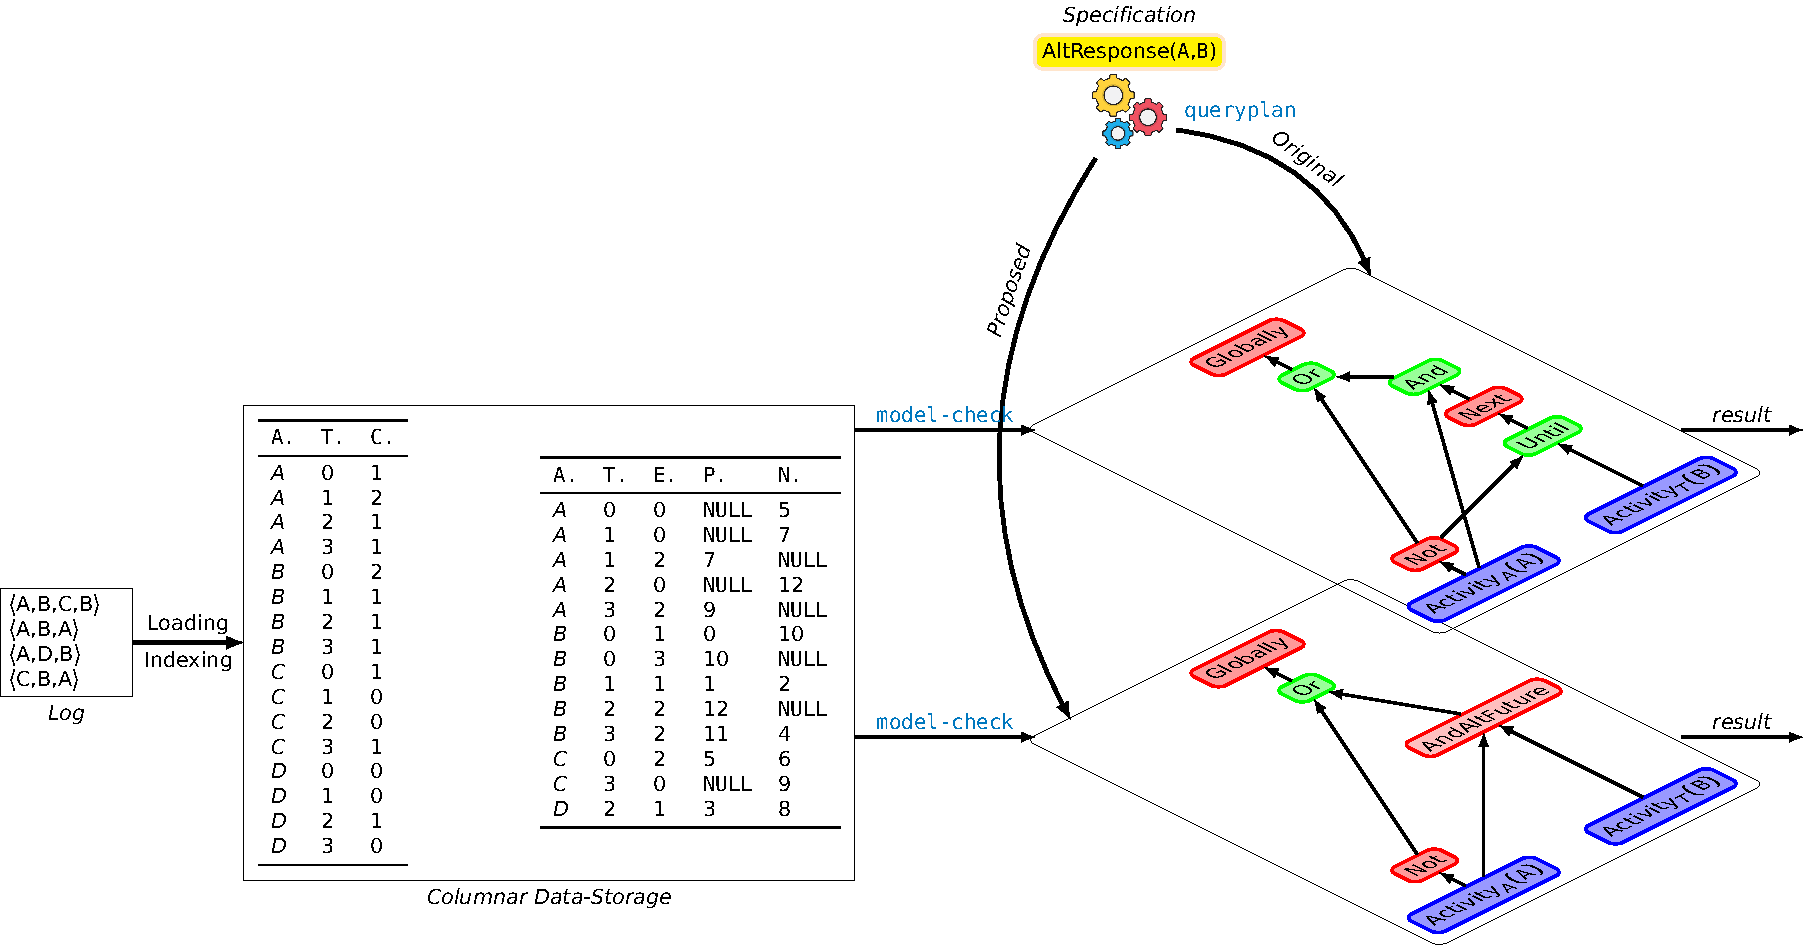
\includegraphics[width=.85\linewidth]{images/workflow_b.pdf}
\caption{{High-level} %MDPI: Figure 1 has moved below where it is first mentioned, please confirm. Giacomo: Added a reference to the figure in the previous paragraph, therefore, I moved this here, where it was first identified
 representation of the KnoBAB query plan for running a $\DeclareClauseNoData{AltResponse}{A}{B}$ for different specifications over a pre-loaded log within a columnar data-storage. After~loading and indexing some traces stored as a log, we obtain a columnar data storage. At~warm-up time, we can specify a \texttt{\color{oceanboatblue}{queryplan}%MDPI: please confirm if the blue color could be removed, plrase check the font color in the whole manuscript
} which, at~formal verification (\texttt{\color{oceanboatblue}{model-check}}) time, converts a Declare specification into a \texttt{xt}LTL\textsubscript{f} query plan. As~KnoBAB supports multiple \texttt{\color{oceanboatblue}{queryplan}}s at once, we can run the same formal verification task over different resulting query plans.}\label{fig1}
\end{figure}

{First}, due to their formulation, some of the logical operators such as the timed until {operator} %MDPI: Please confirm if the special font of variables ``True'' and ``f'' should be retained. There exist many special font in main text in the whole manuscript. Please check whether all of them should be retained or could be removed. Giacomo: The f was fixed, thanks for that.
 \textsc{Until}$^\tau_\textbf{True}(\varphi,\varphi')$ ($\varphi \mathcal{U}\varphi'$ in LTL\textsubscript{f}) are associated with very high computational complexity, as~it prescribes that the occurrence of at least one future event matching a $\varphi'$ condition per trace shall always be preceded by events matching $\varphi$. Under~the occasions that this temporal post-condition shall be considered only after determining the occurrence of a first event  $\varphi''$, this could drastically reduce the amount of computation associated with the overall task. This is not taken into account in our previous implementation in KnoBAB, as~it computed a union between the cases where $\varphi''$ does not occur and the ones where $\varphi''$ occurs, for~which the evaluation of \textsc{Until}$^\tau_\textbf{True}(\varphi,\varphi')$ is extended to any event occurring of the trace. Walking in the footsteps of relational algebra, where $\theta$-joins are expressed as the combination of natural joins~\cite{DBLP:books/mg/AtzeniCPT99} or cross-products~\cite{10.5555/2842853} with $\theta$-selections and join operations can be streamlined through cogrouping~\cite{DBLP:books/x/dittrich2016}, we then propose similarly derived operators, combining the matching of a given pre-condition with the subsequent requirement that all the intermediate events should meet the alternance requirements dictated by \textsc{Until}$^\tau_\Theta$. This paper will then contextualize the need for such derived operators for two specific Declare temporal templates, \textsf{{AltPrecedence}} and \textsf{{AltResponse}}, thus substantiating the interest in these temporal patterns from the current literature (\tablename~\ref{tab:dt}).














\begin{table}[H]\renewcommand{\arraystretch}{1.5}
	\centering
	\caption{{Declare} %MDPI: 1. Table 1 has moved below where it is first mentioned, please confirm. 2. Please confirm if the vertical lines in the table is unnecessary and could be removed.
 \textsf{templates} as exemplifying clauses. $A$ ($B$) represents the \textit{activation} (\textit{target}) condition as an  activity~{label.} %MDPI: We added bold and set the first row as table header, please confirm. Giacomo: that's great, thanks.
}\label{tab:dt}
	\resizebox{\textwidth}{!}{\begin{tabular}{c|lp{9cm}l}
			\noalign{\hrule height 1pt} 
			 & \textbf{Exemplifying Clause (}\boldmath{$c_l$}\textbf{)} & \textbf{Natural Language Specification for Traces} & \textbf{LTL\textsubscript{f} Semantics} \textbf{(}\boldmath{$\llbracket c_l \rrbracket$}\textbf{)}\\
		\noalign{\hrule height 0.5pt} 
				 & \textsf{ChainPrecedence ($A,B$) }  & The activation is immediately preceded by the target. & $\Globally(\Next A\Rightarrow B)$\\ 


			\parbox[t]{2mm}{\multirow{4}{*}{\vspace{10pt}\rotatebox[origin=c]{90}{\textit{In this paper}}}} & \textsf{ChainResponse ($A,B$) }  & The activation is immediately followed by the target. & $\Globally(A\Rightarrow \Next B )$\\
			
			& \textsf{AltResponse ($A,B$) }  & If activation occurs, no other activations must happen until the target occurs.  & $\Globally(A\Rightarrow\Next(\DUntil{\neg A}{B}))$\\
			& \textsf{AltPrecedence ($A,B$) }  & Every activation must be preceded by a target without any other
			activation in between &   $\WeakUntil{\neg B}{A}\wedge \Globally(A\Rightarrow \Next(\WeakUntil{\neg A}{B }))$\\
	\noalign{\hrule height 0.5pt} 
	  \parbox[t]{2mm}{\multirow{13}{*}{\vspace{-40pt}\rotatebox[origin=c]{90}{\textit{Not subject to optimization in this paper}}}}  & \textsf{Init ($A$)} & The trace should start with an activation & $A$\\
	 & \textsf{Exists ($A,n$)} & Activations should occur at least $n$ times & $\Future(A\wedge \Next (\llbracket\textsf{Exists} (A,n-1)\rrbracket)_{n>0})$\\
	 & \textsf{Absence ($A,n+1$)}  & Activations should occur at most $n$ times & $\neg \llbracket\textsf{Exists}$ ($A,n+1$)$\rrbracket$\\
	 & \textsf{Precedence ($A,B$)}  & Events preceding the activations should not satisfy the target & $\WeakUntil{\neg B}{A}$\\
	& \textsf{Choice ($A,A'$) }  & One of the two activation  conditions must appear. & $\Future A\vee\Future A'$ \\
	 & \textsf{Response ($A,B$) } & The activation is either followed by or simultaneous to  the target. & $\Globally(A\Rightarrow\Future B)$ \\
	 & \textsf{RespExistence ($A,B$) }  & The activation requires the existence of the target.& $\Future A\Rightarrow\Future B$ \\
	 & \textsf{ExlChoice ($A,A'$) } & Only one activation condition must happen. & $\llbracket\DeclareClause{Choice}{A}{p}{A'}{p'}\rrbracket\wedge \llbracket\DeclareClause{NotCoExistence}{A}{p}{A'}{p'}\rrbracket$\\ 
	 & \textsf{CoExistence ($A,B$) }  & \textsf{RespExistence}, and~vice~versa. & $ \llbracket\DeclareClauseNoData{RespExistence}{A}{B}\rrbracket\wedge \llbracket\DeclareClauseNoData{RespExistence}{B}{A}\rrbracket$\\
	 & \textsf{Succession ($A,B$) }  & The target should only follow the activation. & $\llbracket\DeclareClauseNoData{Precedence}{A}{B}\rrbracket\wedge \llbracket\DeclareClauseNoData{Response}{A}{B}\rrbracket$\\

	 & \textsf{ChainSuccession ($A,B$) }  & Activation immediately follows the target, and~the target immediately preceeds the activation. & $\Globally(A\Leftrightarrow\Next B)$\\

	 
	& \textsf{NotCoExistence ($A,B$) } & The activation \texttt{nand} the target happen.&  $\neg(\Future A \wedge\Future B)$\\
	 & \textsf{NotSuccession ($A,B$)} & The activation requires that no target condition should follow.& $\Globally(A\Rightarrow \neg\Future B)$ \\
			\noalign{\hrule height 1pt} 
	\end{tabular}}
  \caption*{{\textit{Legend}: Globally: $\Globally\phi$, Next: $\Next\phi$, Implication: $\phi\Rightarrow\phi'$, Until: $\DUntil{\phi'}{\phi}$, Weak Until: $\WeakUntil{\phi}{\phi'}$, Future: $\Future\phi$}.}
\end{table}


\vspace{-20pt}


\begin{Example}
\added{$\DeclareClauseNoData{AltResponse}{A}{B}$ requires that, when \texttt{A} occurs, \texttt{B} shall occur anytime in the future while no other \texttt{A} shall occur in between. %% Giacomo: this text has been changed
In~\texttt{xt}LTL\textsubscript{f}, this can be expressed as $\Globally(\neg\texttt{A} \vee (\texttt{A} \wedge \Next(\DUntil{\neg\texttt{A}}{\texttt{B}})))$ (\textsf{Original} in \figurename~\ref{fig1}). On~the other hand, the~present paper shows that, by~replacing $\texttt{A} \wedge \Next(\DUntil{\neg\texttt{A}}{\texttt{B}})$ with a single operator, we obtain a significant reduction in running time by reducing the amount of result scans and data allocations. This is possible by providing a different (\textsf{Proposed}) \texttt{xt}LTL\textsubscript{f} {queryplan} while implementing \textsf{AndAltFuture} as a novel operator. This difference is remarked in the two resulting query plans in \figurename~ \ref{fig1}.}
\end{Example}








{{Second},} %MDPI: Please confirm if the italics is unnecessary and could be removed. Please check all italics in throughout the paper.
 temporal constraints requiring that events abiding by a $\varphi$ specification shall always precede (or follow) other events abiding by $\varphi'$ are currently implemented in KnoBAB by equi-joining all the events matching  $\varphi$ with the ones matching $\varphi'$, while the predicate is $i=i' \wedge j=j-1$ (or $i=i' \wedge j=j'+1$), where $i$ (or $i'$) and $j$ (or $j'$) are, respectively, referring to the trace id and event id associated to a record coming from the first (or second) operand (see \textsf{And}$^\tau_\Theta$ \texttt{xt}LTL\textsubscript{f} in Section~\ref{xtltlf}). Even this implementation can be further boosted by minimizing the data table access to just one operator (e.g., $\varphi$) for directly accessing the immediately preceding or following events within the relational database and checking whether they abide by $\varphi'$. Even this second observation is motivated by the existence of \textsf{ChainResponse} and \textsf{ChainPrecedence} Declare templates, thus requiring the definition of novel derived operators for performance~purposes.


%outperformed the previous implementation. 



To support our research claims, we extend ({\url{https://github.com/datagram-db/knobab/releases/tag/v2.3}}, Accessed on 7 January 2024) the current implementation of KnoBAB~\cite{computers12090185}, a~column-oriented main memory DBMS supporting formal verification and specification mining tasks by defining relational operations for temporal logic and customary mining algorithms. Despite this being a main memory engine, it currently supports intra-query parallelism and hybrid algorithms (Section~\ref{knobab}). To~our knowledge, no other database management system for temporal formal verification over LTL\textsubscript{f} provides these features, for~which we choose to extend such a system. Furthermore, KnoBAB already proved to consistently outperform previous state-of-the-art algorithms on both tasks~\cite{BurattinMS16}, thus including competing approaches interpreting the same temporal constraints over SQL and row-oriented relational database architecture~\cite{DBLP:conf/caise/SchonigRCJM16}. After~providing a brief literature overview on the landscape of formal verification for temporal data (Section~\ref{sec:relwork}), we outline the following main contributions \added{leading to the our performance analysis result for our newly proposed \texttt{xt}LTL\textsubscript{f} operators}:
\begin{itemize}
\item We formally introduce the novel temporal operators optimizing the aforementioned scenarios in the context of Declare as a declarative language for formal verification (Section~\ref{sec:opdef}).
\item We describe the implementation of the aforementioned operators over the KnoBAB architecture leveraging columnar-oriented main memory storage (Section~\ref{sec:algos}).
\item We present experimental results to evaluate the effectiveness of such newly introduced operators in the context of formal verification in Declare (Section~\ref{sec:empeval}). 
\end{itemize}





\section{Related~Works}\label{sec:relwork}
\unskip
\subsection{Languages for Temporal Formal~Specifications}\label{ssec:languages}
\unskip
\subsubsection{LTL\textsubscript{f}}
Taking the possible worlds as finite traces, LTL\textsubscript{f} is a well-established extension of modal logic with modalities referring to time; it assumes that all the events of interest are fully observable and therefore deterministic and that, for~each occurring event, they should be immediately followed by at most one event. This entails that the $i$-th trace $\sigma^i$ in a log $\LOG$ can be considered as a sequence of $n$ totally ordered events $\sigma^i_0\dots\sigma^i_{n-1}$, where each event $\sigma^i_j$ is associated to a single activity label $\lambda(\sigma^i_j)\in\Sigma$ \cite{DBLP:conf/bpm/BergamiMMM21}.  \added{When events are associated to a payload represented as a key-value association $\varsigma(\sigma^i_j)$, we refer to such logs as \textit{dataful} and as \textit{dataless} otherwise. In~the eventuality of the former, such payloads can be represented as finite functions $V^K$, where $K$ is the set of the keys and $V$ is the overall set of non-\texttt{NULL} values}. \added{C}oncerning our datasets of interest, we only consider %are going to consider similar 
ones where trace events are not associated with a data payload, and~therefore even such logs can be considered as \textit{dataless}. \added{On the other hand, with~reference to \cref{ourLog}, event payloads can store patient information, thus registering the recorded medical condition being observed~\cite{info14030173}; in the context of good brokerage, such payload might contain the relevant contract information between the supplier and the customer which are required to be respected (e.g., delivery times), as~well as the location of the goods, their number, and~quality~\cite{DBLP:conf/wbdb/PetermannJMR14}.}


LTL\textsubscript{f} semantics is usually defined in terms of First-Order Logic~\cite{DBLP:conf/tamc/ZhuPV19}; more informally, \texttt{Next} ($\Next\phi$) requires $\phi$ to occur from the subsequent temporal step, \texttt{Globally} ($\Globally\phi$) that $\phi$  always holds from the current instant of time, \texttt{Future} ($\Future\phi$)  that $\phi$ must eventually hold, and~ \texttt{Until} $\DUntil{\phi}{\phi'}$ that $\phi$ must hold until the first occurrence of $\phi'$ does. {W}%MDPI: We removed the bold here, please confirm.
eak Until is a \textit{derived operator} for ${\varphi}\mathcal{W}{\varphi'}:={\varphi}\mathcal{U}{\varphi'}\vee\Globally{\varphi}$, while the logical implication can be rewritten as $\varphi\Rightarrow\varphi':=(\neg \varphi)\vee (\varphi\wedge \varphi')$. \added{Please observe that LTL\textsubscript{f} does not provide full support for handing data correlation conditions between operands of binary operations, as~it only supports the declaration of data conditions that can be applied to one single event~\cite{DBLP:conf/bpm/BergamiMMM21}. To~the best of our knowledge, \texttt{xt}LTL\textsubscript{f} (Section~\ref{xtltlf}) is the only extension of this language supporting data payload correlation across events matched by both arguments of the binary operator, thus providing a complete \textit{dataful} support.}


\subsubsection{Declare} 

Declare~\cite{4384001,Li2020} provides a human-readable declarative language on top of LTL\textsubscript{f} (first column  of Table~\ref{tab:dt}), where each template is associated with a specific LTL\textsf{f} formula (third column), which can be instantiated with arbitrary activity labels. We refer to the instantiation of such templates via activity labels in a finite set $\Sigma$ as \textit{(declarative) clauses}. Declare circumscribes the set of all the possible behaviors expressible in LTL\textsubscript{f} to the ones of interest over a set of possible  $\Sigma$; Table~\ref{tab:dt} recalls some of the most used templates while remarking on the four templates of interest optimized in the present~paper. 


 At the time of writing, Declare expresses specifications $\spec$ as a set of clauses $c_l$ being usually associated with an LTL\textsubscript{f} semantics $\llbracket c_l\rrbraket$; in this context, a~trace $\sigma\in\LOG$ satisfies a Declare specification $\spec$ if it jointly satisfies all the clauses associated to the specification. If~these clauses can be characterized by a precondition which, if~satisfied by some event, imposes the occurrence of a post-condition, then we refer to these as \textit{activation} and \textit{target} conditions, respectively. Please observe that post-conditions are considered as such merely in terms of causal implication (i.e., $\Rightarrow$) and not necessarily in temporal terms, e.g.,~while \textsf{ChainResponse} requires the target to immediately follow any existing activation, \textsf{ChainPrecedence} requires that the targeted event shall instead precede the activation. Please consider that Declare clauses do not necessarily reflect association rules, as~the latter do not provide temporal constraints correlating the activation of activation and target conditions. In~this paper, we focus on Declare clauses only predicating over the events' activity labels, which are then referred to as \textit{dataless}\deleted{considering our datasets of interest, we are going to consider similar dataset where trace events are not associated with a data payload, and~therefore even such logs can be considered as \textit{dataless}}; on the other hand, \textit{dataful} Declare clauses can express  data payload conditions over both activation and target conditions, as~well as representing $\Theta$ payload correlation conditions between activating and targeted conditions~\cite{info14030173}. Thus, both clauses and logs are referred to \textit{dataful} otherwise. 

Despite the fact that the four clauses of interest in \tablename~\ref{tab:dt} might appear to express similar behavior, they express substantially different concepts. \tablename~\ref{btable} provides four traces distinguishing the behavior of such four templates, the validity of which can be easily controlled by transforming the associated LTL\textsubscript{f} formul\ae~ into a DFA ({\url{http://ltlf2dfa.diag.uniroma1.it/dfa}}, Accessed on \mbox{7 January 2024)}.






\begin{table}[H]
\caption{{Traces} %MDPI: 1. Table 2 has moved below where it is first mentioned, please confirm. 2. Please confirm if the hook and cross in the table need explanations. 3. We added bold and set the first row as table header, please confirm.
 \added{from the Log in \figurename~\ref{fig1}} distinguishing the temporal behavior of the Declare clauses of interest in this paper, where each trace $\sigma^i_0\dots\sigma^i_{n-1}$ is expressed in terms of their associated activity labels, $\braket{\lambda(\sigma^i_0),\dots, \lambda(\sigma^i_{n-1})}$. \cmark  (and \xmark) remarks a trace satisfying (violating) a corresponding clause.  }\label{btable}
\centering
	\begingroup % trick algorithm2e into thinking we're in one column mode
	\csname @twocolumnfalse\endcsname
	\noindent
	\resizebox{\textwidth}{!}{%
		\begin{minipage}{1.2\textwidth}\begin{tabular}{lcccc}
\toprule
     \textbf{Traces} & \pmb{\texttt{ChainResponse}(\textsf{A,B})} &\pmb{\texttt{ChainPrecedence}(\textsf{B,A})} &\pmb{ \texttt{AltResponse}(\textsf{A,B}) }& \pmb{\texttt{AltPrecedence}(\textsf{B,A})}\\
\midrule
    $\braket{\textsf{A,B,C,B}}$ & \cmark & \xmark & \cmark& \xmark \\
    $\braket{\textsf{A,B,A}}$& \xmark & \cmark & \xmark& \xmark \\
    $\braket{\textsf{A,D,B}}$ & \xmark & \xmark & \cmark& \xmark\\
    $\braket{\textsf{C,B,A}}$ & \xmark & \xmark & \xmark & \cmark \\
\bottomrule
\end{tabular}		\end{minipage}%
	}% <------------- end of \resizebox
\endgroup
\end{table}










\subsection{KnoBAB and \texttt{xt}LTL\textsubscript{f}}
\textit{{We}%MDPI: Please confirm if the italics is unnecessary and could be removed. Please check all italics in throughout the paper.
~now summarize our previous contributions on temporal formal verification tasks run over our proposed main memory columnar database, KnoBAB.}

\subsubsection{KnoBAB}\label{knobab}
\textit{KnoBAB} \cite{info14030173,computers12090185} is a column database store tailored for both loading \textit{dataful} logs being represented in XES~\cite{DBLP:journals/cim/AcamporaVSAGV17} and \textit{dataless} ones described as a tab-separated file. This outperformed the previous state of the art in terms of both specification mining~\cite{APrioriDeclare} and formal verification~\cite{BurattinMS16} tasks on tailored non-database~solutions.  

\paragraph{Logical and Physical Model} 

The resulting column-based relational database is then represented through some tables having fixed schema independently from its data representation. As~the present paper focuses on dataless datasets, we describe in this paper just two of those; \tablename~\ref{atable} describes the relational representation of the log presented in Equation~(\ref{ourLog}). 
The ActivityTable (\tablename~\ref{atable}a) lists each trace event of a given log, where records are sorted in ascending order for activity label, trace id, and~event id. Cells under the  \texttt{Prev} (and \texttt{Next}) column store a pointer to the record representing the immediately preceding (and following) event in the same trace if any. After~mapping each existing activity label in the log $\const{a}$ to a unique natural number $\beta(\const{a})$, we can define a primary dense and clustered index  that can be accessed in $O(1)$ time as it is an array of offset pointers. We also define a secondary index structured as a block of two records, associating each trace in the log to the  first and last trace event; given that all the traces are associated with a unique natural number, this index can also be accessed on $O(1)$ time by trace id. The~CountTable (\tablename~\ref{atable}b), also created at loading time like the previous, merely lists the number of occurrences of each activity label per trace and can be used to determine the absence or presence of an event with a given activity label per~trace.




\paragraph{Formal Verification Tasks over Query Plans} In spite of the ActivityTable also appearing in SQLMiner's log representation~\cite{DBLP:conf/caise/SchonigRCJM16} (except for the \texttt{Prev} and \texttt{Next} columns), this still used an off-the-shelf relational database engine and a translation of Declare specification into SQL for carrying out formal verification tasks over a dataless log. KnoBAB showed a new pathway for enhancing temporal queries over customary main memory relational database through the combined provision of both ad~hoc  relational operators expressing LTL\textsubscript{f} over relational tables (\texttt{xt}LTL\textsubscript{f}) and the definition of a query plan represented as a rooted DAG where shared subqueries are computed only once~\cite{BellatrecheKB21}. This was sensibly different from competing approaches~\cite{DBLP:books/sp/22/MurillasRA22,DBLP:books/sp/22/KammererPR22} also relying on main memory engines where, instead, the~query plan associated to a formal verification task is always expressed in terms of trees, thus not allowing the detection of shared sub-expressions to be merged to avoid wasteful recomputations. As~vertices for a DAG can be sorted topologically, we can obtain for free the scheduling order in which the operators must be executed and, by~associating each node a maximum distance value from the root, we can safely run in parallel all the operators laying at the same depth level, as all the previously called operators will pertain their information in an intermediate cache, thus achieving intraquery parallelism as a free meal~\cite{info14030173}. This parallelization approach greatly differs from straightforward parallelization algorithms known in the Business Process Management area, where they simply run each declarative clause occurring in the specification in a separate thread~\cite{BurattinMS16}. In~addition to the former, KnoBAB guarantees efficient access to the tables through the provision of specific indexing data structures such as primary indices for directly accessing the blocks of the table concerning a specific activity label as well as the provision of secondary indices mapping a specific trace id $i$ and event id $j$ for $\sigma^i_j$ into a table offset. KnoBAB outperformed SQLMiner run over PostgreSQL within two to five orders of magnitude, thus demonstrating the inadequacy of using customary relational operators for computing temporal tasks over relational~databases. 





\begin{table}[H]
\caption{{KnoBAB} %MDPI: 1. Table 3 has moved below where it is first mentioned, please confirm. 2. we merged the two sub-tables into one and also revised their citations in mian, please confirm. 3. We added bold and set the first row as table header, please confirm.
 representation for the dataless log in Equation~(\ref{ourLog}). (\textbf{a}) ActivityTable; (\textbf{b}) CountTable.}\label{atable}



\begin{tabular}{>{\raggedright\arraybackslash}m{3.5cm}>{\raggedright\arraybackslash}m{2cm}>{\raggedright\arraybackslash}m{2.2cm}>{\centering\arraybackslash}m{2cm}>{\centering\arraybackslash}m{2cm}}
\toprule
\multicolumn{5}{c}{({\textbf{a}})}   \\
\midrule
    \pmb{\texttt{ActivityLabel}} & \pmb{\texttt{TraceId}} &\pmb{ \texttt{EventId}} &  \pmb{\texttt{Prev}} & \pmb{\texttt{Next}}\\





\midrule
    {{Clinical Test} %MDPI: Please confirm if the italics is unnecessary and can be removed. Same in the whole text.
} & 1 &  2 & 7 & 5\\
    {Discharge} & 0 & 2 & 4 & \texttt{NULL}\\
    {Discharge} & 1 &  4 & 5& \texttt{NULL}\\
    {Discharge} & 2 &  3  & 6& \texttt{NULL}\\
    {Examination} & 0 & 1 & 9 & 1\\
    {Examination} & 1 &  3 & 0& 2\\
    {Examination} & 2 &  2 &8&3\\
    {Redirection} & 1 & 1 & 10 & 0 \\
    {Redirection} & 2 & 1 & 11 & 6\\
    {Registration} & 0 & 0 & \texttt{NULL} & 4\\
    {Registration} & 1 &  0 & \texttt{NULL} & 7\\
    {Registration} & 2 &  0 & \texttt{NULL} &  8\\
\midrule
\multicolumn{5}{c}{({\textbf{b}})}   \\
\midrule
     \pmb{\texttt{ActivityLabel}} & \pmb{\texttt{TraceId}} & \pmb{\texttt{Count}}\\
\midrule




    {Clinical Test} & 0 &  0&&\\
    {Clinical Test} & 1 &  1&&\\
    {Clinical Test} & 1 &  0&&\\
    {Discharge} & 0 & 1&&\\
    {Discharge} & 1 & 1&&\\
    {Discharge} & 2 & 1&&\\
    {Examination} & 0 & 1&&\\
    {Examination} & 1 &  1&&\\
    {Examination} & 2 &  1&&\\
    {Redirection} & 0 & 0&&\\
    {Redirection} & 1 & 1&&\\
    {Redirection} & 2 & 1&&\\
    {Registration} & 0 & 1&&\\
    {Registration} & 1 &  1&&\\
    {Registration} & 2 & 1&&\\
\bottomrule
\end{tabular}


\end{table}






%\texttt{\color{red} Other competing approaches also not expressing the query plan as a DAG, but rather as a tree, thus not benefitting from computing the same sub-expressions shared across clauses at most once while also not providing minimal data access to the tables: }

KnoBAB enables the specification of user-defined template names in terms of \texttt{xt}LTL\textsubscript{f} operators through a {\color{oceanboatblue}{\texttt{queryplan}}  ~{\texttt{``semantics\-name'' \{}\ldots\texttt{\}}}} query, thus allowing the co-presence of multiple possible definitions of declarative clauses. Then, we can select the most appropriate semantics while carrying out the formal verification task by specifying such a name, e.g.,~{\color{oceanboatblue}{\texttt{model-check}}~{\ldots \texttt{plan ``semanticsname''} \ldots}} This then enables us in this paper to test multiple possible specifications of Declare clauses without necessarily recompiling the database's source~code.


Walking in the footsteps of the BAT algebra for columnar databases~\cite{IdreosGNMMK12}, each of the novel temporal operands for \texttt{xt}LTL\textsubscript{f} (Section~\ref{xtltlf}) not requiring direct data access to the aforementioned KnoBAB tables both accepts as an input and returns a uniform data representation \added{$\rho$} with schema:
\begin{equation}\label{schema}
 \texttt{IntermediateRepresentation}(\texttt{TraceId},\texttt{EventId},\texttt{Witnesses(Tag)})
\end{equation}
 where the first (and second) argument refers to the trace (and event) id matching a specific temporal condition of choice, while \texttt{witnesses} \added{represents the relevant} activated or targeted conditions occurring from the position \texttt{EventId} in a given \texttt{TraceId} trace onwards \added{via  a tagged extension of semiring provenance~\cite{10.1145/1265530.1265535}}; \added{such tags mainly refer to} the distinction between activated and targeted events\deleted{is made explicit with appropriate tags}, respectively $A$ and $T$. Dataful matching occurring between witnessed activated $A(i)$ and targeted events $T(j)$ certified via a $\Theta$ binary predicate are represented as $M(i,j)$. \added{Matches can be represented as semiring products, while the listing of all the activated, targeted, and~matched events can be represented as a semiring sum; the latter is simply rendered as a list.}
 As the table is sorted by trace id and event id by design for any given activity label, such intermediate representation  also returns  trace entities sorted by ascending trace id and event id.


\subsubsection{\texttt{xt}LTL\textsubscript{f}}\label{xtltlf}
\textit{We now discuss some \texttt{xt}LTL\textsubscript{f} operators of relevance for the current paper. By~using KnoBAB as a computational model, we can also discuss the time complexity associated with such operators.} While LTL\textsubscript{f} operators can mainly be used to establish a yes/no question about whether a single trace abides by some temporal specification, an~\texttt{xt}LTL\textsubscript{f} expression returns all the traces in the log conforming to a temporal specification by composing the trace events as records through temporal operations. Furthermore, the~latter can also be directly exploited to express confidence, maximum satisfiability, and~support metrics similar to association rules. So to better support future explainable temporal AI tasks, \texttt{xt}LTL\textsubscript{f} also carries out information concerning activated/targeted events justifying the algorithmics' outcome, while the cache associated to the leaves can be analyzed so as to check which events were activated/targeted without necessarily satisfying the temporal requirements computed through \texttt{xt}LTL\textsubscript{f}.

\paragraph{Table Access (``Leaf'') Operators} We  determine all the events being associated with a specific activity label through the ActivityLabel's primary block index and express the outcome of this retrieval in terms of intermediate representation:
\[ \textsf{Activity}^{\LOG,\tau}_{A/T}(\const{a})=\{\braket{i,j,\{A/T(j)\}}|\exists \pi,\phi.\braket{\const{a},i,j,\pi,\phi}\in\textsf{ActivityTable}\}\]
where $A/T$ provides the optional tags for remarking the matching event of interest as being part of an activation/target condition. By~associating each activity label \const{a} with a unique natural number $\beta(\const{a})$, we can now seek the presence of events with label \const{a} in $O(1)$ time and retrieve all the events $\#{\textsf{a}}\ll |\LOG|$ associated to such a label. If, on~the other hand, we are interested in events matching a specific data predicate $q$,  we define the following operator:
\[\textsf{Atom}^{\LOG,\tau}_{A/T}(\textsf{B},q)=\{\braket{i,j,{A/T(j)}}\;|\;q(\sigma^i_j)\wedge \lambda(\sigma^i_j)=\textsf{B}\}\]
Despite the fact that this might appear as a simple selection operation, the~atomization of a predicate into mutually exclusive data conditions required for both minimizing the data access to the tables holding the key-value payload associations within the dataful events and merging multiple equivalent sub-expressions into one makes both its associated query plan and its actual formal definition quite convoluted. As~describing this is not the major purpose of the paper, we refer to~\cite{info14030173}
 for any further information. %Despite this, which might resemble the selection predicate from traditional relational algebra at first glance, the~atomization of each key-value correspondence as a distinct table requires additional technical details. Due to the data minimisation access, its formulation is not straightforward. Please observe that its detailed formal specification requires additional knowledge on the representation of the AttributeTables which, due to the lack of space, are not discussed in the present paper but can be found in~\cite{info14030173}. 
By accessing the secondary index of the \textsf{ActivityTable}, we can collect the last events for each trace in linear time over the log's size $O(|\LOG|)$ using the following operator:
\[\textsf{Last}^{\LOG,\tau}_{A}=\{\braket{i,\vert\sigma^i\vert,\{A(\vert\sigma^i\vert)\}}|\exists \const{a}, \pi.\braket{\beta(\const{a}),i,|\sigma^i|,\pi,\texttt{NULL}}\in\textsf{ActivityTable}\}\]

\paragraph{Unary Operators} 

We discuss the main difference between  operators' execution in  \texttt{xt}LTL\textsubscript{f} from corresponding ones in LTL\textsubscript{f}; the latter computes semantics from the first occurring operator appearing in the formula towards the leaves, whereas the former assumes intermediate results coming from the leaves. In~this, the~downstream operator is completely agnostic about the semantics associated with the upstream operator, so it must combine the intermediate results appropriately. Therefore, the~\textsf{Next}$(\rho)$ (timed) \texttt{xt}LTL\textsubscript{f} unary operator returns all the events $\sigma^i_j$ witnessing the satisfaction of an activation, target, or~correlation condition being returned by a downstream operator as an intermediate result $\rho$, while $\Next\varphi$ will simply increment the internal time counter over $\varphi$, thus determining the time from which to assess the specification in $\varphi$.

Due to this structural discrepancy in the order of computation, \texttt{xt}LTL\textsubscript{f} must distinguish \textit{timed} operators (assessing the occurrence of a specification sub-expression anytime in the trace) from the \textit{untimed} operators (determining the properties holding from the beginning of the trace). The~aforementioned \texttt{xt}LTL\textsubscript{f} operator can therefore be expressed as follows:
\[\textsf{Next}^\tau(\rho)=\Set{\braket{i,j-1,L}|\braket{i,j,L}\in\rho,j>0}\]
This operator can then be computed in linear time over the size of the input, i.e.,~$O(|\rho|)$.
On the other hand, the~timed negation operator $\textsf{Not}^\tau(\rho)$ subtracts from the universal relation, being all the \added{events occurring in any trace}, the \textsf{ActivityTables} events appearing in $\rho$ while still guaranteeing the return of the records in ascending order for trace and event id. Given $\epsilon$, the maximum trace length, this operator takes at most $O(|\LOG|\epsilon)$ time by assuming $|\rho|\ll |\LOG|\epsilon$. The~globally timed operator prescribes to return a $\braket{i,j,L}\in\rho$ if also all the subsequent events within the same trace are in $\rho$, and~can be computed in $O(|\rho| \log|\rho|)$ time by starting scanning the events from the last occurring in the~trace.  

\paragraph{Binary Operators} 

We now stress further differences between \texttt{xt}LTL\textsubscript{f} and LTL\textsubscript{f} in terms of binary operators. While \texttt{xt}LTL\textsubscript{f} can  express dataful matching conditions between activation and target conditions,  LTL\textsubscript{f} can only express properties associated with one single event at a time through atoms.
In these regards, timed logical conjunction ($\textsf{And}^\tau_\Theta(\rho,\rho')$) extending the logical conjunction in LTL\textsubscript{f} with a binary match condition $\Theta$ over the event's payloads can be expressed as a nested $\Theta$-join returning the records from both operands having the same trace id and event id, while all the pairs of witnessed events satisfying an activation $A(i)$ and target $T(j)$ conditions from the matching record shall satisfy the $\Theta$ matching condition when provided; the matching is then registered with $M(i,j)$. Timed logical disjunction ($\textsf{Or}^\tau_\Theta(\rho,\rho')$) can be similarly expressed through a full outer $\Theta$-join. Given that the ActivityTable is pre-sorted at indexing time, we can efficiently implement such algorithms through sorted joins. As~these can be computed with a joint linear scan of both operands, both operators have at most a time complexity in $O(|\rho|+|\rho'|)$. The~timed until operator ($\textsf{Until}^\tau_{\textbf{True}}(\rho,\rho')$) {for} %MDPI: please confirm if the bold of ``true'' is unnecessary and could be removed here. Please check all bold throughout the paper.
 $\Theta=\textbf{True}$ is defined similarly to the corresponding LTL\textsubscript{f} operator; it returns all the events within a given log trace in the second operand and the events from the first operand if all the immediately following events until the first occurrence of an event in the second operand also belong to the first:
		\[\begin{split}
 			\textsf{Until}^\tau_\textbf{True}(\rho,\rho')=\rho'\cup \Set{\langle i,k,L\cup L'\rangle |\exists j>k. \braket{i,j,L}\in\rho', 
(\forall k\leq h<j. \braket{i,h,L'}\in\rho) }
\end{split}\]
This can be computed in $O(|\rho|^2|\rho'|)$ time in its worst-case scenario.
 The in-depth discussion concerning the formal definition of such an operator when matching a non-trivially true matching condition $\Theta$ is deferred due to its technicalities and can be retrieved from the original paper~\cite{info14030173}.


\subsection{Algebraic Specification for~Queries}\label{timecompl}
\textit{We now compare \texttt{xt}LTL\textsubscript{f} with other long-standing definitions of temporal operators regarding database temporal representations.} 

\added{Current research~\cite{DBLP:conf/caise/SchonigRCJM16} outlined the possibility of loading logs composed of multiple traces within row-based relational databases while providing a direct translation of \textit{dataless} Declare-driven formal verification and specification mining tasks into SQL~\cite{Schonig15}. Our previous research remarked on the inefficiency of directly expressing temporal formal verification tasks on top of off-the-shelf relational databases, thus motivating the definition of a novel query plan specification directly exploiting temporal algebra operators, \texttt{xt}LTL\textsubscript{f} \cite{info14030173}. As~SQL queries are translated into query plans where each operator expresses an implementation of a relational algebra operator, this demonstrates the overall inefficiency of exploiting traditional relational algebra for representing temporal queries.} Please observe that LTL\textsubscript{f} temporal requirements cannot be expressed in traditional relational algebra without aggregation operators while not naturally assuming a columnar database storage. Therefore, \added{traditional relational algebra} cannot be directly exploited to predicate about the necessity or the eventuality of a given event to occur without any further~extension.

For all these considerations, our proposed algebra more resembles BAT from MonetDB~\cite{IdreosGNMMK12,DBLP:journals/pvldb/BonczMK09}, where the intermediate result output for each operator records the table's record being selected, without necessarily carrying out values stored within the specific row. Given the specificity of our scenario, our intermediate results carry the trace id and the event id as unique record identifiers. We further had to extend this representation to possibly carry out the activated and targeted events as witnesses of the computation's correctness, providing explainable justifications for the computation, and~correctly expressing $\Theta$ predicates over dataful logs. \texttt{xt}LTL\textsubscript{f} then provides a required extension of such a representation for new computation~needs.

Concerning Allen's algebra for temporal intervals~\cite{10.1145/182.358434}, we can \textit{first} see that such algebra considers events as temporal intervals that might also be overlapping, while \texttt{xt}LTL\textsubscript{f} inherits the same assumptions from LTL\textsubscript{f} and considers events as pointwise and non-overlapping activities. \textit{Secondly}, while the former only supports conditions on the activity labels, \texttt{xt}LTL\textsubscript{f} also supports predicating on the conditions for the payload values (expressed as key-value pairs) associated with the specific events~\cite{info14030173}, as~well as supporting binary predicates to be tested across activated and targeted conditions similarly to $\theta$-joins. Recent extensions of Allen's algebra aimed at supporting single data conditions over single events~\cite{DBLP:books/sp/22/MurillasRA22}. \textit{Thirdly}, such algebra only expresses temporal correlations between two single events, albeit expressed with a duration and a termination time, and~can predicate \added{natively} neither the eventuality nor the necessity of some properties to occur in a trace (e.g., globally and future) from a given instant in~time.

Concerning the temporal relational algebra~\cite{DBLP:conf/cikm/Wang95} defined over temporal relational databases~\cite{DBLP:series/txcs/Revesz10} (also referred to as \textit{temporal modules} \cite{DBLP:journals/isci/WangJS95}), it mainly   proposes timestamp transformation operations \added{currently supported by Oracle Cloud~\cite{oraclecloud}} as well as windowing functions, thus retaining the entities and relationships occurring within a window time frame. \added{This allows the slicing of a temporal module into a finite sequence of finite database states, where such a snapshot sequence can be ascribed to a single trace and each event can be mapped to a single database state~\cite{tuzhilin2018using}.} Despite time being considered as a first citizen within these operators, no operator of such an algebra temporally correlates entities at different timestamps while also requiring the eventuality or the necessity for a specific condition within a given lapse of time. 
\deleted{Please observe that LTLf temporal requirements cannot be expressed in traditional relational algebra without aggregation operators while not naturally assuming a columnar database storage. Therefore, this algebra cannot be directly be exploited to predicate about the necessity or the eventuality of a given event to occur without any further extension.} \added{An orthogonal contemporary approach attempted at mapping LTL\textsubscript{f} to TSQL2~\cite{10.1007/BFb0014161}, a~de facto extension of SQL for querying temporal modules~\cite{Snodgrass2009}. Differently from the approach mentioned above, this preserved LTL\textsubscript{f} temporal operators such as Until ($\mathcal{U}$); as the authors preceded the definition of LTL\textsubscript{f} extensions considering data payload conditions~\cite{DBLP:conf/bpm/BergamiMMM21,info14030173}, these are not considered in their transformation. Furthermore, as~these temporal modules represent one single distinct trace as a result of temporal snapshotting of a single database into multiple distinct states, they cannot be effectively used to run a single formal verification task over numerous traces as per our proposed approach, as~this would require running a single TSQL2 query over multiple databases, one for each log trace. In~fact, our solution can assess multiple traces simultaneously by leveraging an extended relational representation to the one initially described in~\cite{DBLP:conf/caise/SchonigRCJM16}.}


\deleted{For all these considerations, our proposed algebra resembles more BAT from MonetDB, where the intermediate result output for each operator records the table's record being selected without necessarily carrying out values stored within the specific row. Given the specificity of our scenario, our intermediate results carry the trace id and the event id as unique record identifiers. We further had to extend this representation to possibly carrying out the activated and targeted events as witnesses of the computation's correctness, providing explainable justifications for the computation, and~correctly expressing $\Theta$ predicates over dataful logs. \texttt{xt}LTLf then provides a required extension of such representation for new computation needs.}

%unique record identifiers are split into two distinct identifiers, a trace id and an event id. Nevertheless, this representation had to be extended due to the correlation conditions expressible in Declare, where any two events in the trace might have been correlated temporally. This therefore required the aforementioned extension of witnessing events within the intermediate representation format.



\section{Proposed Derived~Operators}\label{sec:opdef}
\textit{{Similarly} %MDPI: Please confirm if the italics is unnecessary and could be removed. Please check all italics in throughout the paper.
 to the definition of the derived operators in relational algebra, we now provide the definition of our proposed operators extending \texttt{xt}LTL\textsubscript{f} by expressing those in terms of the ones already known in such a temporal algebra. These are then defined in \cref{AAF,AAW,eq:andNext,lastEQ}. %The next section will provide greater details on how such operators, being here formalised in terms of existing operators for simplicity's sake, can be actually implemented as self-standing operators from scratch.
}


\subsection{{AndAltFuture} %MDPI: we revised into 2nd-level heading, please confirm. same below in this section.
} 

We want this operator to seek all the instants of time when an event activates the Declare clause while the target  follows anytime in the future, while requiring that no further activation occurs between these two events. This operator aims  to optimize the \textsf{AltResponse(A,B)} clause and can be then expressed in terms of basic \texttt{xt}LTL\textsubscript{f} operators as {follows:} %MDPI: please confirm if the blue color could be removed, plrase check all the font color in the whole manuscript

\begin{equation}\label{AAF}
{\color{oceanboatblue}\textsf{AndAltFuture}^\tau_\Theta(\rho,\rho')}\eqdef\textsf{And}^\tau_\Theta\bigg(\rho,\textsf{Next}\Big(\textsf{Until}^\tau_\textbf{True}\big(\textsf{Not}^\tau(\rho),\rho'\big)\Big)\bigg)
\end{equation}

By implementing this operator from scratch, we want to avoid running the costly computation of the timed \textsf{Until}$^\tau$ unless the activation condition associated with the intermediate result returned as $\rho$ is satisfied. Furthermore, we want to avoid explicitly computing the negation of the activation condition and express this by explicitly checking that, given any activating event in $\sigma^i_j$ in $\rho$ with an immediately following targeting one $\sigma^i_{k}$ in $\rho'$ with $|\sigma^i|>k>j$, no other events $\sigma^i_{j+h}$ in $\rho$ with $j+h<k$ shall occur. We can then express the aforementioned Declare clause in terms of the recently defined operator as follows:
\begin{equation}\label{qp1}
\textsf{Globally}^\tau\Big(\textsf{Or}^\tau_\textbf{True}\big(\textsf{Not}^\tau(\rho),{\color{oceanboatblue}\textsf{AndAltFuture}^{\tau}_{\textbf{True}}(\rho,\rho')}\big)\Big)
\end{equation}
where $\rho=\textsf{Activity}^{\LOG,\tau}_A(\textsf{A})$ and $\rho'=\textsf{Activity}^{\LOG,\tau}_T(\textsf{B})$ under the dataless~assumption.


\begin{Example}
\added{With reference to the log in Equation~(\ref{ourLog}), $\DeclareClauseNoData{AltResponse}{redirect}{examine}$ requires that a patient redirected to a given department shall be examined before being further redirected. This constraint satisfies all the traces within that equation. By~considering only the events from the second trace, in~our previous \texttt{xt}LTL\textsubscript{f} solution we have intermediate results $\rho=\textsf{Activity}_A(\texttt{redirect})=\{\braket{1,1,[A(1)]}\}$ for the activation condition and $\rho'=\textsf{Activity}_T(\texttt{examine})=\{\braket{1,3,[T(3)]}\}$ for the target one.  The~timed Until  $\rho''=\textsf{Until}^\tau_\textbf{True}(\neg\rho,\rho')$ returns:}
 \[\{\braket{1,0,[T(1)]},\dots,\braket{1,3,[T(3)]},\braket{1,4,[]}\}\]

\added{as each event in \texttt{xt}LTL\textsubscript{f} can only witness a future event, and~$\rho'''=\textsf{Next}^\tau(\rho'')$ returns:}
 \[\{\braket{1,1,[T(3)]},\dots,\braket{1,2,[T(3)]},\braket{1,3,[]}\}\]

\added{Hence, $\textsf{And}_\textbf{True}^\tau(\rho,\rho''')$ returns just $f=\{\braket{1,1,[M(1,3)]}\}$, while witnessing that, from~that time onwards, both activation $A(1)$ and target $T(3)$ condition will occur from the same event $1$. The~rest of the events will be returned via $\neg\rho$, which are finally grouped-by temporally via untimed \textsf{Globally}. Before~running it, we previously ran the timed Until operator independently from the occurrence of $\rho''$ in a trace. }

\added{On the other hand, our new \textsf{AndAltFuture} operator directly returns $f$ after taking as an argument $\rho$ and $\rho'$; this scans the events in $\rho'$ occurring after each occurrence of events in $\rho$ while immediately discarding the events in $\rho$ containing another redirect event in between. This reduces the memory footprint and the number of scans from our previous query plan.}
\end{Example}

\subsection{AndAltWFuture} 


Reflecting upon the definition of \textsf{AltPrecedence\-(A,B)} which this operator is aiming to optimize, we can observe that implementing an ad~hoc operator AndAltWFuture for this might provide even greater optimization, as~we might as well avoid checking the global absence of \textsf{A}-labelled events if no \texttt{B} occurs in a trace after an \textsf{A}. Therefore, this operator acts as an extension of the former by either requiring an alternate occurrence between activation and target condition, as previously, or requiring the absence of any future activation if no targeting event is expected to occur. $\color{oceanboatblue}\textsf{AndAltWFuture}^\tau_\Theta(\rho,\rho')$ can be then defined as follows:
\begin{equation}\label{AAW}
\textsf{And}^\tau_\Theta\Bigg(\rho,\textsf{Next}\bigg(\textsf{Or}^\tau_\textbf{True}\Big(\textsf{Until}^\tau_\textbf{True}\big(\textsf{Not}^\tau(\rho),\rho'\big),\textsf{Globally}^\tau\big(\textsf{Not}^\tau(\rho)\big)\Big)\bigg)\Bigg)
\end{equation}
We can now express \textsf{AltPrecedence(A,B)} by replacing, in~the original \texttt{xt}LTL\textsubscript{f} Declare semantics, the~previous equation with the currently introduced operator, thus obtaining:
\begin{equation}\label{qp2}
    \begin{split}
\textsf{Or}^\tau_{\textbf{True}}\Bigg(&\textsf{Until}^\tau\Big(\textsf{Not}^\tau(\rho'),\rho\Big),\textsf{Globally}^\tau\bigg(\textsf{Or}^\tau_\textbf{True}\Big(\textsf{Not}^\tau(\rho),{\color{oceanboatblue}\textsf{AndAltWFuture}^{\tau}_{\textbf{True}}(\rho,\rho')}\bigg)\Bigg)\\
\end{split}
\end{equation}


\subsection{AndNext} 

This operator aims to optimize the \textsf{ChainResponse} operator by reducing the data access by accessing the \texttt{ActivityTable} just for the activation condition. This makes this operator intrinsically unary, as~the target condition, both in terms of data predicate and activity label, has to be provided as additional arguments for the operator alongside the $\Theta$ correlation condition for dataful scenarios. To~check whether the target condition occurs immediately after the operand's current event, we need to check whether it is associated with an activity table and whether it satisfies a predicate $q$. This can be then expressed in \texttt{xt}LTL\textsubscript{f} in terms of the following derived operator:
\begin{equation}\label{eq:andNext}
{\color{oceanboatblue}\textsf{AndNext}^\tau_{\textsf{B},q,\Theta}(\rho)}\eqdef\textsf{And}^\tau_\Theta\left(\rho,\textsf{Next}^\tau(\textsf{Atom}^{\LOG,\tau}_{T}(\textsf{B},q))\right)
\end{equation}
At this stage, we can then express the semantics associated to the Declare template \textsf{ChainResponse(A,B)} as follows:
\begin{equation}\label{qp3}
    \textsf{Globally}^\tau\left(\textsf{Or}^\tau_\textbf{True}\left(\textsf{Not}^\tau(\rho),{\color{oceanboatblue}\textsf{AndNext}^{\LOG,\tau}_{B,\textbf{True},\textbf{True}}(\rho)}\right)\right)
\end{equation}
where $\rho=\textsf{Activity}^{\LOG,\tau}_A(\textsf{A})$ in a dataless scenario.



\subsection{NextAnd} 

The second operator aims at optimizing \textsf{ChainPrecedence(A,B)} similarly to the previous one, but~with a swapped temporal occurrence. Please observe that negating the fact that an event shall occur after another can be expressed in terms of all the events occurring at the end of a trace and all of the events not matching the activation condition a when occurring in a non-first position. So, ChainPrecedence is usually represented as:
\[\begin{split}
\textsf{Globally}^\tau\Bigg(\textsf{Or}^\tau_\textbf{True}\bigg(&\textsf{Or}^\tau_\textbf{True}\Big(\textsf{Last}^{\LOG,\tau},\textsf{Next}^\tau(\textsf{Not}^\tau(\rho))\Big), {\color{oceanboatblue}\textsf{And}^\tau_\textbf{True}\Big(\textsf{Next}^\tau(\rho),\rho'\Big)}\bigg)\Bigg)
\end{split}\]
where $\rho=\textsf{Activity}^{\LOG,\tau}_A(\textsf{A})$ and $\rho'=\textsf{Activity}^{\LOG,\tau}_T(\textsf{B})$ in a dataless scenario. After~compactly representing the subexpression in the second row of the previous definition, as follows:
\begin{equation}\label{lastEQ}
{\color{oceanboatblue}\textsf{NextAnd}^\tau_{\textsf{B},q,\Theta}(\rho)}\eqdef\textsf{And}^\tau_\Theta\left(\textsf{Next}^\tau(\rho),\textsf{Atom}^{\LOG,\tau}_{T}(\textsf{B},q)\right)
\end{equation}
 we %then therefore substitute it with this newly-defined derived operator.\medskip
aim to optimize this last declarative clause by using this last introduced operator by rewriting the semantics associated to \texttt{Chain\-Precedence}(\textsf{A},\textsf{B}) as such:
\begin{equation}\label{qp4}
    \begin{split}
\textsf{Globally}^\tau\Bigg(\textsf{Or}^\tau_\textbf{True}\bigg(&\textsf{Or}^\tau_\textbf{True}\Big(\textsf{Last}^{\LOG,\tau},\textsf{Next}^\tau\big(\textsf{Not}^\tau(\rho)\big)\Big),{\color{oceanboatblue}\textsf{NextAnd}^\tau_{\textsf{B},\textbf{True},\textbf{True}}(\rho)}\bigg)\Bigg)
\end{split}
\end{equation}
Please observe that the intended optimization induced by these operators can be considered as non-trivial, as~these do not directly subsume the entire \texttt{xt}LTL\textsubscript{f} semantics associated to a template, rather than optimizing a specific~part.


\section{Algorithmic~Implementation}\label{sec:algos}
\textit{{We}%MDPI: Please confirm if the italics is unnecessary and could be removed. Please check all italics in throughout the paper.
~discuss the implementation of the previously introduced operators outlined in Algorithm \ref{algo:fdgt}, thus justifying their definition as novel derived operators. For~each of them, we briefly discuss their computational complexity and compare it to the expected theoretical speed-up not considering the cost of memory allocation and page-faults.}\medskip

%%%%%%%%%%%%%
\begin{algorithm}[H]
	\begingroup % trick algorithm2e into thinking we're in one column mode
	\csname @twocolumnfalse\endcsname
	\noindent
	\resizebox{\textwidth}{!}{%
		\begin{minipage}{1.4\textwidth}
\begin{algorithmic}[1]


\Function{AndAltFuture$^\tau_\Theta$}{$\rho,\rho'$}
\ForAll{$\braket{i,j,L},\braket{i,k,L'}\in (\rho\times \rho')$ \textbf{s.t.} $j< k$ }\label{actualLinearScan}

\If{$\not\exists h>0. \braket{i,j+h,L}\in\rho$ \textbf{s.t.} $j+h<k$ }\label{notActivation1}
%\State {$L''\gets \bigcup\{\tilde{L}|\braket{i,h,\tilde{L}}\in\rho',h\geq k\}$}
\If{$L'\neq\emptyset$ \textbf{and} $L\neq\emptyset$ \textbf{and} $\Theta\neq \textbf{True}$}
\State $L''\gets\{M(j',k')|\Theta(\sigma^i_{j'},\,\sigma^i_{k'}),A(j')\in L, T(k')\in L'\}$
\State \algorithmicif\; $L''\neq\emptyset$ \algorithmicthen\; \textbf{yield} $\braket{i,j,L''}$\label{matchingForEvents}
\Else\; \textbf{yield} $\braket{i,j,L\cup L''}$\label{morcheeba}
\EndIf
\EndIf
\EndFor
\EndFunction
\Statex
\Function{AndAltWFuture$^\tau_\Theta$}{$\rho,\rho'$}
\ForAll{$\braket{i,j,L} \in \rho$  }
\ForAll{$\braket{i,k,L'}\in \rho'$ \textbf{s.t.} $j\leq k$}
\If{$\not\exists h>0. \braket{i,j+h,L}\in\rho$ \textbf{s.t.} $j+h<k$ }\label{notActivation2}
\State \algorithmicif\; $j=|\sigma^i|-1$ \textbf{continue};
%\State {$L''\gets \bigcup\{\tilde{L}|\braket{i,h,\tilde{L}}\in\rho',h\geq k\}$}
\If{$L\neq\emptyset$ \textbf{and} $L'\neq\emptyset$ \textbf{and}  $\Theta\neq \textbf{True}$}
%\State $L''\gets\{M(j,k+h)|\Theta(\sigma^i_{j'},\,\sigma^i_{k+h}),A(j')\in L, T(k+h)\in L''\}$
\State $L''\gets\{M(j',k')|\Theta(\sigma^i_{j'},\,\sigma^i_{k'}),A(j')\in L, T(k')\in L'\}$
\State \algorithmicif\; $L''\neq\emptyset$ \algorithmicthen\; \textbf{yield} $\braket{i,j,L''}$
\Else\; \textbf{yield} $\braket{i,j,L\cup L''}$
\EndIf
\EndIf
\EndFor
\If{$\not\exists k,h. \braket{i,k,L'}\in \rho'\wedge \braket{i,h,L''}\in \rho\wedge j< k,j<h$}\label{weakness}
\State \textbf{yield} $\braket{i,j,L}$\label{withAbsenceActivationOnwards}
\EndIf
\EndFor
\EndFunction

\Statex
\Function{AndNext$^\tau_{\textsf{B},q,\Theta}$}{$\rho$}
\State \algorithmicif\; $\not\exists \sigma^i\in\LOG,\sigma^i_j\in\sigma^i. \lambda(\sigma^i_j)=\textsf{B}$ \algorithmicthen\;\Return $\emptyset$\label{countScan}
\ForAll{$\braket{i,j,L}\in \rho$ \textbf{s.t.} $j<|\sigma^i|-1$ \textbf{and} $\lambda(\sigma^i_{j+1})=\textsf{B}$ }\label{firstCond}
\State $L'\gets L\cup\{T(j+1)\}$
\If{$\Theta\neq\textbf{True}$}
\State \algorithmicif\; $L\neq\emptyset$ \textbf{and} $\not\exists A(k)\in L. \theta(\sigma^i_k,\,\sigma^i_{j+1})$ \algorithmicthen\; \textbf{continue}
\State \algorithmicelse\; $L'\gets \{M(k,j+1)|A(k)\in L\}$\label{hasMatch1}
\EndIf
\State \algorithmicif\; $q\neq\textbf{True}\vee q(\sigma^i_{j+1})$ \algorithmicthen\; \textbf{yield} $\braket{i,j,L'}$ \label{actualReturn1}
\EndFor
\EndFunction
\Statex
\Function{NextAnd$^\tau_{\textsf{B},q,\Theta}$}{$\rho$}
%\State \algorithmicif\; $\not\exists \sigma^i\in\LOG,\sigma^i_j\in\sigma^i. \lambda(\sigma^i_j)=\textsf{B}$ \algorithmicthen\;\Return $\emptyset$
\ForAll{$\braket{i,j+1,L}\in \rho$ \textbf{s.t.} $j\geq 0$ \textbf{and} $\lambda(\sigma^i_{j})=\textsf{B}$ }
\State $L'\gets L\cup\{T(j)\}$
\If{$\Theta\neq\textbf{True}$}
\State \algorithmicif\; $L\neq\emptyset$ \textbf{and} $\not\exists A(k)\in L. \theta(\sigma^i_k,\,\sigma^i_{j})$ \algorithmicthen\; \textbf{continue}
\State \algorithmicelse\; $L'\gets \{M(k,j)|A(k)\in L\}$
\EndIf
\State \algorithmicif\; $q\neq\textbf{True}\vee q(\sigma^i_{j})$ \algorithmicthen\; \textbf{yield} $\braket{i,j+1,L'}$
\EndFor
\EndFunction

\end{algorithmic}
		\end{minipage}%
	}% <------------- end of \resizebox
	\endgroup


 \caption{Newly proposed \texttt{xt}LTL\textsubscript{f} operators.}\label{algo:fdgt}
\end{algorithm}



\subsection{{AndAltFuture} %MDPI: we revised into 2nd-level heading, please confirm. same below in this section.
} 







As all the intermediate results in the KnoBAB pipeline are always sorted by ascending trace and event id, we can scan all the events within the same trace where the targets follow the activations in linear time similarly to the timed \textit{and} operator, despite this being expressed in pseudocode with a cross product for simplifying the overall notation ({Line} %MDPI: We revised ``L.'' into ``Line'', please confirm all.
 \ref{actualLinearScan}). We then consider all the events in the same trace having no immediate subsequent event in $\rho$ prior to the occurrence of the next event in $\rho'$; this can be simply checked in $\rho$ by determining that the next record appearing in $\rho$ after $\braket{i,j,L}$ has an event id less than $k$ ({Line} \ref{notActivation1}). If~there is a non-trivially true $\Theta$ predicate, we also impose that at least one activation occurring after or at $\sigma^i_j$ and at least one target occurring after or at $\sigma^i_k$ matches with $\Theta$ ({Line} \ref{matchingForEvents}). Otherwise, we compute no match, and~we straightforwardly collect the activation and target conditions from both events ({Line} \ref{morcheeba}). In~the code, we explicitly injected an early-stopping condition avoiding testing subsequent events in $\rho'$ within the same trace as soon as we detect one event in $\rho$, invalidating the condition at {Line} \ref{notActivation1}. By~considering the time complexities for each \texttt{xt}LTL\textsubscript{f} operator in Section~\ref{timecompl}, we can argue that the time complexity associated with computing this operator as in the previous section without the aforementioned computation is totalled to $O(|\rho|+(||\LOG||-|\rho|)^2|\rho'|+2((||\LOG||-|\rho|)+|\rho'|))$, where $||\LOG||=|\LOG|\epsilon$. On~the other hand, by~assuming to always scan each trace quadratically of length $\epsilon$ for each event in $\rho$, we obtain the time complexity of $O(|\rho|\sfrac{\epsilon^2}{2}+|\rho'|)$ for the derived operator when implemented as per the previous discussion. If~we assume that $\rho$ and $\rho'$ are associated with a single activity label, as per the scenario in Declare, where the number of events and the activity labels are uniformly distributed such that $\# \textsf{a}\approx \sfrac{|\LOG|\epsilon}{|\Sigma|}$ for each $\textsf{a}\in\Sigma$, we can derive that the provided algorithm always provides a positive speed-up if compared to the original formulation in Equation~(\ref{AAF}). 

\subsection{AndAltWFuture} 
This algorithm works similarly to the previous, where we relax the until condition with a weak until, thus also admitting an absence of activation conditions after the first occurrence (of an activation) if no further target events are present ({Line} \ref{weakness}). Even in this scenario, we have a similar time complexity to the previous, while the original formulation in Equation~(\ref{AAW}) introduced an additional overhead to the previous by computing an additional timed disjunction and the global computation over the negation of the possibly activating events. Therefore, we expect an even greater speed up for this latest~operator.   

\subsection{AndNext} 

As previously observed in the formal definition of this operator, we transformed this into an unary operator where, instead of retrieving two sets of events associated with two activity labels, we just scan one of the two. Before~starting any form of scan, we immediately return if, after~a $O(|\LOG|)$ scan of the CountTable, we detect that no event is associated with the target condition ({Line} \ref{countScan}). Otherwise, we consider only events both coming from traces containing an event with  activity label \texttt{B} and not being at the end of the trace, and~for which the immediately next event is associated to an activity label {\texttt{B}} %MDPI: please confirm if the bold  is unnecessary and could be removed here. Please check whether it should also add ``\texttt{}'' to keep it uniform in main. 
 as a target condition ($T(j+1)$, {Line} \ref{firstCond}); we implementationally further enhanced this by completely skipping any test whether the event resides in a trace where no \texttt{B} event resides. If~$\Theta\neq\textbf{True}$, then we also have to guarantee that each activation condition appearing in $\rho$ should match with the target event at time $j+1$ ({Line} \ref{hasMatch1}) and, upon~provision of $q$, the~target condition should also match with this ({Line} \ref{actualReturn1}). The~computational complexity of this operator is in $O(|\rho|+|\LOG|)$ and, if~we are taking into account the accessing time to the immediately following event, if any, we obtain a time in $2|\rho|+|\LOG|$. If~compared to the time complexity of Equation~(\ref{eq:andNext}) of $|\rho|+2|\rho'|$, we then obtain a positive speed up, i.e.,~$\frac{|\rho|+2|\rho'|}{2|\rho|+|\LOG|}> 1$, for~$|\rho'|>\sfrac{|\rho|}{2}$ and $0<|\LOG|<2|\rho'|+|\rho|$.  

\subsection{NextAnd} 

This other operator works similarly to the previous, where we are checking instead the immediately preceding event instead of looking at the immediately following one, thus requiring that each element of interest in $\rho$ shall never be at the beginning of the trace. The~same considerations over speed-up and time complexity follow from the previous algorithm. %, thus obtaining a positive speed-up with $\frac{|\rho|+2|\rho'|}{2|\rho|}\geq 1$ for $0<|\rho|\leq 2|\rho'|$ and $|\rho'|>0$.  
\medskip

After associating each of the novel operators in the aforementioned algorithmic implementation,  \cref{qp1,qp2,qp3,qp4} will then provide the semantics generating the query plan as \texttt{Proposed} in this current paper, while the direct translation of the LTL\textsubscript{f} expressions in \tablename~\ref{tab:dt} to the operators outlined in Section~\ref{xtltlf} provides the \texttt{Original} formulation of the query plan also in~\cite{info14030173}, where none of the previous algorithms are~used.



%we then generate a new query plan, where the sub-expressions from Equation~(\ref{AAF})-\ref{lastEQ} were completely replaced with the corresponding \texttt{xt}LTL\textsubscript{f} operators and associated algorithms discussed in this section, we then kept the original declarative semantics from (\texttt{Original}) with the one proposed in this paper (\texttt{Proposed}).


\section{Empirical~Evaluation}\label{sec:empeval}





\textit{{Given} %MDPI: Please confirm if the italics is unnecessary and could be removed. Please check all italics in throughout the paper.
~that the aim of our derived operators is to enhance formal verification tasks conducted over temporal clauses expressed in Declare, we compare the different running times of carrying out formal verification tasks over our previous set of operators as well as by replacing those with our currently proposed derived ones, while focusing on benchmarking formal verification tasks over specifications written in Declare. We discard from our evaluation the benchmark of the single operator, as~this is insufficient to remark on their adequacy in enhancing formal verification tasks in Declare. Thus, we compare different query plans being generated from different Declare semantics being specified at runtime through the \texttt{queryplan ``name'' \{} \ldots \texttt{\}} query.  %benchmark the time required for formal verification tasks when such clauses are used rather than benchmarking the running time for each operator. In~fact, given the overall pipeline, we might overall provide an optimisation for such a task providing a minimal overhead to the overall query plan computation. Therefore, 
With this, achieving a positive speed-up in Declare formal verification tasks as in our previous work~\cite{info14030173} by using the proposed operators will tell us that, under~specific data conditions, the~original \texttt{xt}LTL\textsf{f} query plan associated with the declarative clauses available in KnoBAB constitutes the major computational bottleneck. Having a negligible speed-up will likely remark  other components in the query plan dominating the overall running time, while having a negative speed-up only on specific data conditions will motivate some future work on hybrid algorithms, thus allowing us to choose between different algorithms for specific temporal operators depending on the data distribution within the loaded dataset~\cite{DBLP:journals/spe/Musser97}.} 


Our benchmarks exploited a Dell Mobile Precision Workstation 5760 on Ubuntu 22.04: Intel® Xeon(R) W-11955M CPU @ 2.60 GHz $\times$ 16, 64 GB DDR4 3200 MHz RAM. We took two real-world datasets and a synthetic one for our experiments, both being dataless. The~first real dataset ({Hospital}) monitors the patient flow and different medical procedures to which the patients in question were subjected; each trace tracks a single patient from his hospitalization to dismissal, and~each activity label describes the name associated to such phases~\cite{https://doi.org/10.4121/uuid:d9769f3d-0ab0-4fb8-803b-0d1120ffcf54}. The~second one ({Cybersecurity}) provides the auditing step of different malware, where each trace represents  a single malware being audited, while each activity label identifies one single system call event being audited as invoked by the malware~\cite{10.7717/peerj-cs.346,DBLP:conf/siu/YaziCG19}.  The~synthetic dataset was derived from temporal graphs generated by {FoodBroker} \cite{DBLP:conf/wbdb/PetermannJMR14} while describing trades and shipments of goods  mediated by a brokerage company. For~each \texttt{GraphTransaction}, we sort all the vertices describing an event occurring at a specific \texttt{date}, thus also including  \texttt{creation} timestamps. For~vertices describing a ticket being filed by a client raising a complaint, we return an activity label associated with the type of complaint (\texttt{problem}); otherwise, we keep the original vertex label. We then collect the set of temporally ordered activity labels and represent those as log traces. The~updated FoodBroker codebase for generating event logs is also available online (\url{https://github.com/jackbergus/foodbroker/}, Accessed on 7 January 2024).




For each dataset, we then obtain the sampled trace length distribution, and~we sample sub-logs of various sizes while trying to abide by the trace distribution from the original dataset, notwithstanding their skewness. For~the first and third (or second) datasets, we sample the logs so that their sizes are powers of ten (or nine) while always guaranteeing that each sub-log $|\LOG_h|=10^h$ (or $|\LOG_h|=9^h$) is always a subset of any larger sub-log. We also keep the original log as the last sample dataset. This random sampling mechanism is required to better assess the scalability of the proposed operator's implementation while guaranteeing an approximation of the original trace length distribution across the board to guarantee similar running time conditions. \figurename~\ref{fig:PDF} reports the sample PDF trace length for each of the sampled logs alongside the size of each sample. The~{FoodBroker} synthetic dataset contains the shorter traces (\figurename~\ref{fig:PDF}a); all the sampled logs except the first one have a maximum trace length of $24$, while the first sublog has a maximum trace length of $21$. On~the other hand, the~first two smaller log samples of the real-world {Hospital} dataset (\figurename~\ref{fig:PDF}b) have traces with a maximum length of $1200$, while the remaining two have a maximum trace length of $1814$. The~{Cybersecurity} dataset (\figurename ~\ref{fig:PDF}c) contains the longest traces, having a maximum trace length of {$1.23\times10^6$} %MDPI: We revised the center dot to ×, please confirm.
 for the smaller two sub-logs and of {$1.76\times 10^6$} for the remaining ones. This information will soon become relevant while conducting our following analysis of the algorithmic speed-ups given by our proposed derived operators while performing formal verification over the models described in the following~paragraph.






\begin{figure}[H]

\subfloat[\centering]{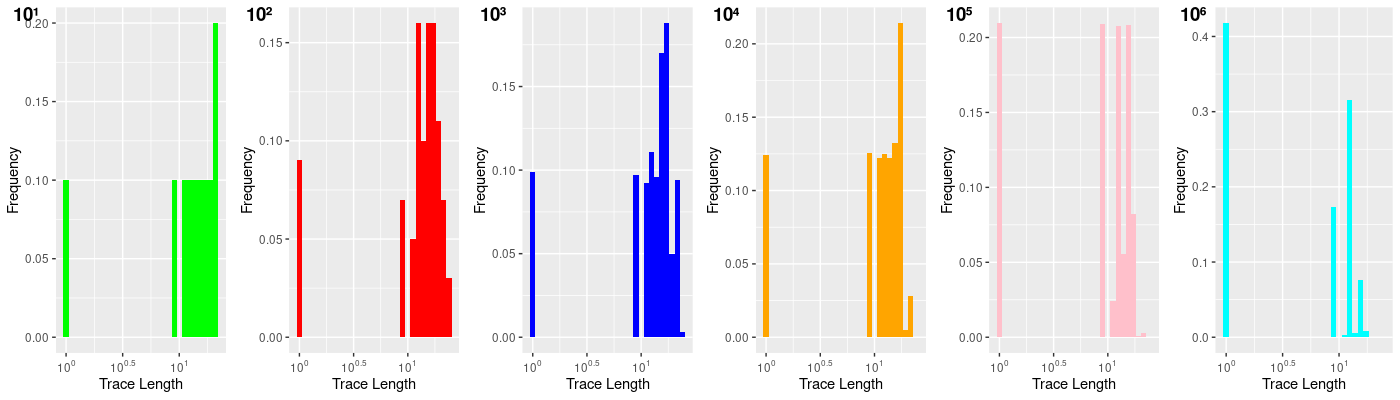
\includegraphics[width=\textwidth]{images/BrokerPDF.png}}

\subfloat[\centering]{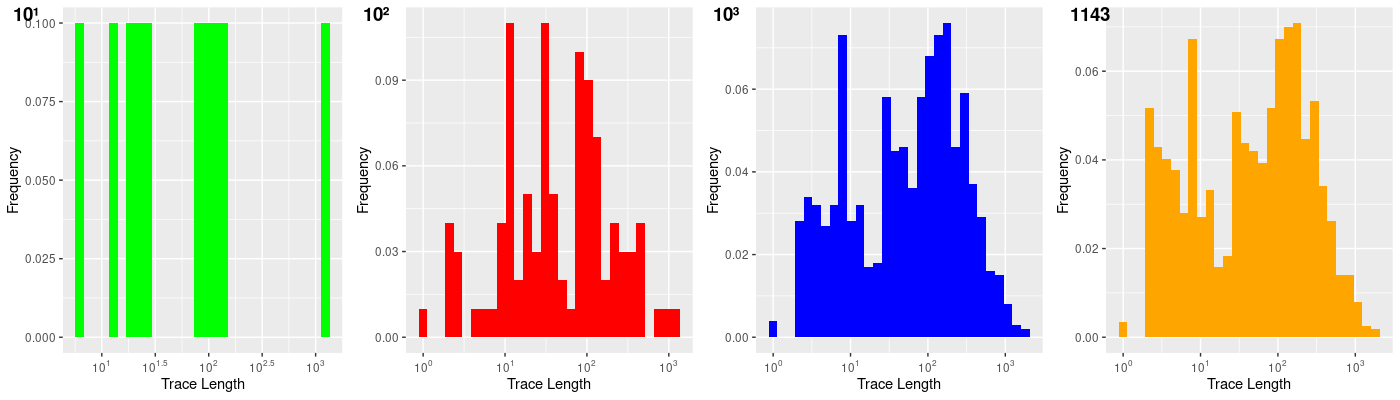
\includegraphics[width=\textwidth]{images/HospitalPDF.png}}

\subfloat[\centering]{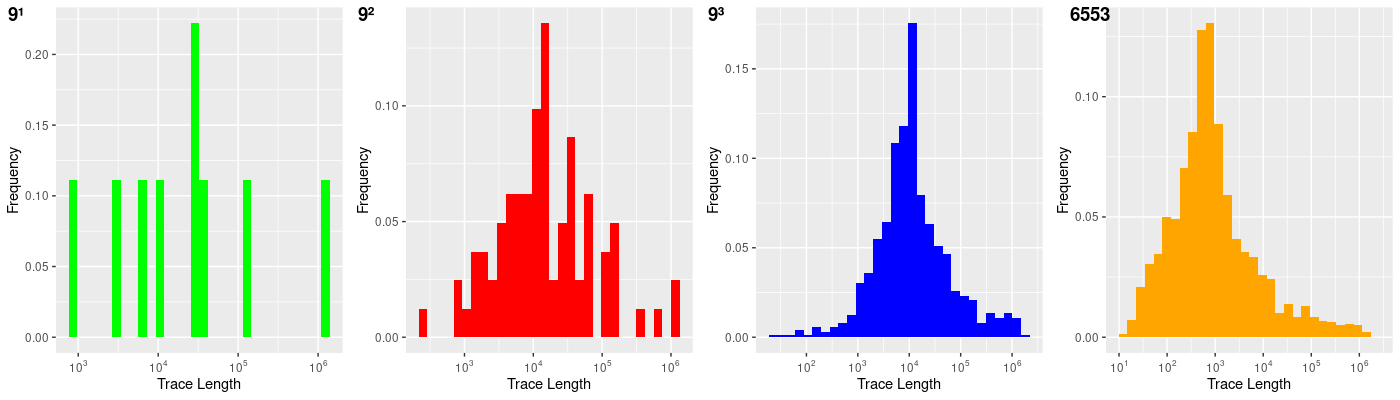
\includegraphics[width=\textwidth]{images/CyberPDF.png}}

\caption{{Sampled} %MDPI: 1. We moved explanations of sub-images into the caption, please confiirm. 2. Please confirm whether different colors in the image need explanations. 3. Figure 2 has moved below where it is first mentioned, please confirm.
 probability density function associated with the length of the traces for each sub-log extracted from each original~dataset: (\textbf{a}) FoodBroker, (\textbf{b}) Hospital,  and (\textbf{c}) Cybersecurity.}\label{fig:PDF}
\end{figure}












 Given that we aim to test these newly introduced \texttt{xt}LTL\textsubscript{f} operators in the context of a Declare-based formal verification task when \texttt{xt}LTL\textsubscript{f} is used to represent its semantics, we generate four specifications $\Phi^c_1,\dots,\Phi^c_4$ for each declarative clause of interest $c$, \textsf{AltPrecedence}, \textsf{AltResponse}, \textsf{ChainPrecedence}, and~\textsf{Chain\-Response}, where each $\Phi^c_i$ contains exactly $i$ binary clauses determined by instantiating an activity label among the most frequently occurring ones within the smaller sub-log. We then use the same specifications generated for the smaller log and the greater sub logs, thus comparing the running times for each sub-log over the same Declare specifications. We then use the specifications to conduct a formal  verification task via a {\color{oceanboatblue} {\texttt{model-check}\ldots}}  query. The~resulting logs and specifications are freely available online (\url{https://osf.io/6y8cv/}, Accessed on 7 January 2024). 

Last, as~our previous work already showed that computing such queries on top of relational databases such as PostgreSQL with shorter traces leads to a greater running time than running similar queries over KnoBAB, we just focus on comparing the results from our previous implementation with the ones after applying the changes discussed in this paper.
\medskip

With reference to Figure~\ref{overallBenchmarks}, {AndAlt}%MDPI: please confirm whether the symbol ``\ding{83}'' here should change into an asterisk. Same highlight below.
\ding{83} operators 
can be deemed responsible for evidently outperforming the proposed query plan if compared to the one from the previous implementation,
%are the ones being more 
%consistently outperform our previous Declare query plan  
as they lead to an associated speed-up  always strictly greater than one. Our previous definition of the Declare operators is greatly affected by the number of clauses within the model, which becomes even more apparent when the maximum and average trace length $\epsilon$ per sampled log increases. On~the other hand, running our former formal verification query plan for {AndAlt}\ding{83} clauses  over the Cybersecurity dataset always took more than one 1H ({$3.6\times 10^6$} ms), thus demonstrating an increased running time for the original query plan strategy when longer traces occur. We stopped recording the running time, as~the overhead introduced by the intermediate operators for carrying out the actual matching between activation and target conditions was strikingly evident, while our proposed operators could instead carry out the formal verification task within one minute. Although~no out-of-memory exceptions were observed before the timeout, these were clearly observed in larger specifications and log sizes, thus clearly demonstrating KnoBAB's limits as a main memory engine by not maintaining the query intermediate results in secondary memory. Despite the code allowing the clearing of intermediate caches to be run to free extra memory, this only partially addresses the out-of-memory failure for larger specifications. %We also obtain similar out-of-memory errors by giving the original operators a sufficient amount of time to compute. 
Overall, this demonstrates that this proposed extension for {AndAlt}\ding{83} operators outperforms our previous query plan definition, as~also expected from our previous analysis concerning the overall theoretical time~complexity.




\begin{figure}[H]


\subfloat[\centering]{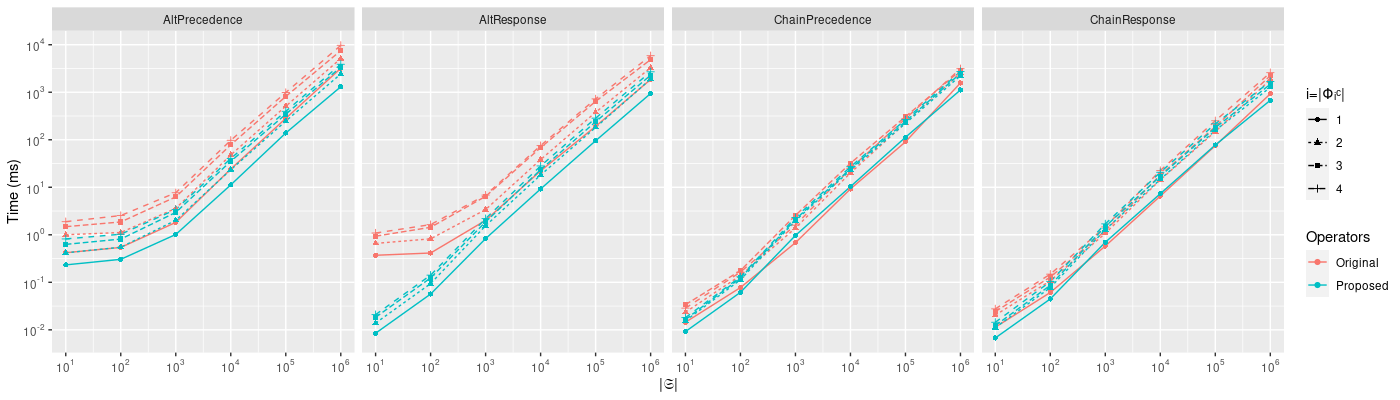
\includegraphics[width=\textwidth]{images/FoodBroker.png}}

\subfloat[\centering]{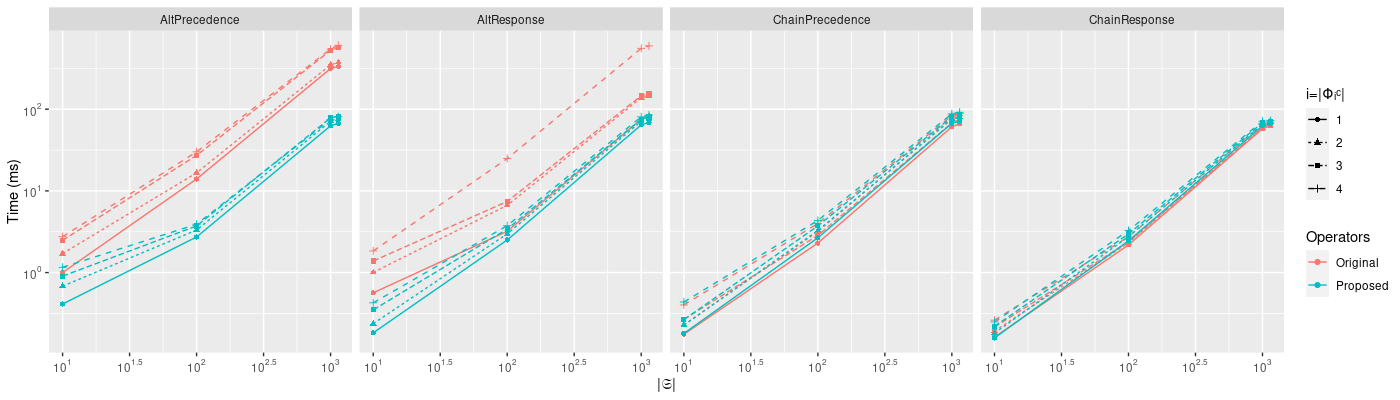
\includegraphics[width=\textwidth]{images/Hospital.png}}

\subfloat[\centering]{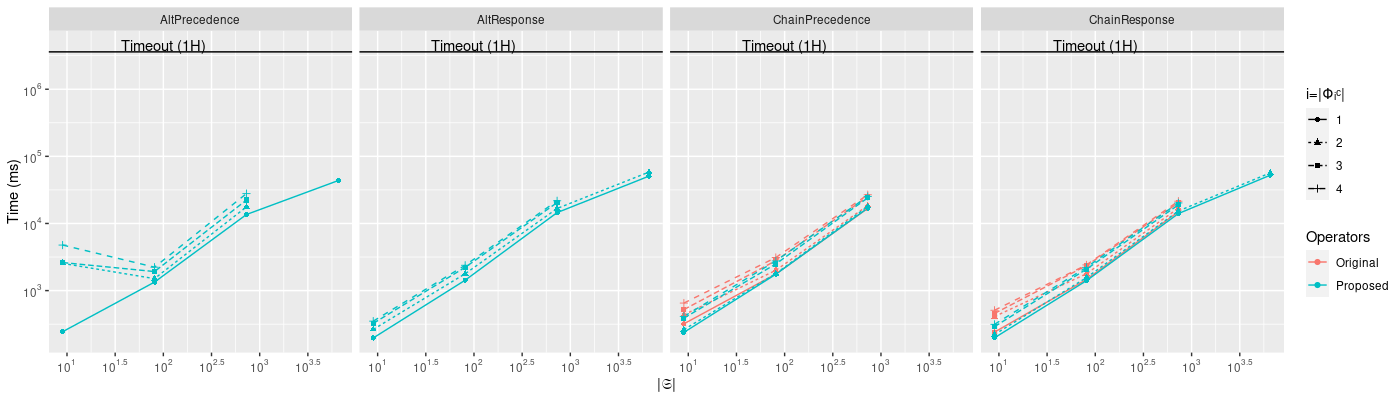
\includegraphics[width=\textwidth]{images/Cyber.png}}


\subfloat[\centering]{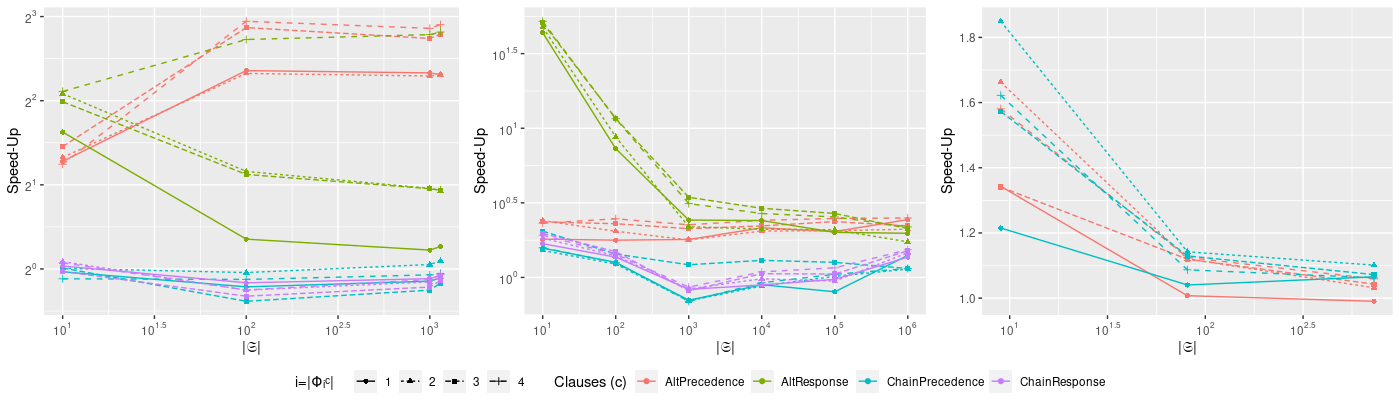
\includegraphics[width=\textwidth]{images/Speedups.png}}


\caption{{Comparing} %MDPI: 1. We moved explanations of sub-images into the caption, please confiirm. 2. Please change the hyphen (-) that represents the negative sign into a minus sign ($-$). 3. Figure 3 has moved below where it is first mentioned, please confirm.
 the proposed implementation of the derived operators with the previous implementation given in~KnoBAB. (\textbf{a}) FoodBroker dataset; (\textbf{b}) Hospital dataset;  (\textbf{c}) Cybersecurity dataset. (\textbf{d}) Datasets' speed-up: (\textbf{{left}%MDPI: We revised the italics to bold format, please confirm.
}) FoodBroker, (\textbf{{center}}) Hospital, and~(\textbf{{right}}) Cybersecurity.}\label{overallBenchmarks}
\end{figure}


{Chain}\ding{83} operators provide a more convoluted scenario to be examined carefully. First, we observe a clear trend correlating datasets with longer traces with an overall increase in speed-up. In~fact, the~{Hospital} datasets exhibit more speed-ups compared to the {FoodBroker} one, where the recently proposed operators yield comparable or underperforming running times. Notwithstanding the former, we can clearly observe that the recently proposed operators consistently outperform our previous solution over the {Cybersecurity} dataset. Differently from our previous set-up, we can now observe that the original formulation of the declarative clauses without the currently presented operators now runs out of memory before hitting the 1H timeout for the larger sample, being the full dataset, while our solution still manages to carry out some temporal formal verification tasks over specifications containing fewer clauses. Last, we consistently observe that such operators still provide greater speed-ups over datasets with smaller log sizes, thus providing theoretical validation to our speed-up equations for such operators. This postulates the need for such operators while dealing with massive datasets, while advocating the usage of hybrid algorithms for switching between the previous solution and the currently proposed~one.


%\texttt{\color{red}[TODO: mainly discuss the experiments' outcome]}

\section{Conclusions and Future~Works}
This paper proposes an extension to our previous work on KnoBAB by optimizing our previously proposed query plan by introducing novel algebraic temporal operators expressing formal verification tasks on column database storages in main memory. As~a consequence, we extended our temporal algebra \texttt{xt}LTL\textsubscript{f} with four novel operators, subsuming entire \texttt{xt}LTL\textsubscript{f} expressions which before could only be represented in terms of combinations of costly basic operators. %This is addressed through the definition of novel derived operators, that is, operators that can be expressed as a combination of already-existing \texttt{xt}LTL\textsubscript{f} operators being a calque of the customary LTL\textsubscript{f} operators. 
Preliminary results over such operators provide non-negligible speed-up to the formal verification tasks over realistic datasets, where several events are audited and collected in a larger collection of~traces. 

Despite these experiments demonstrating the efficiency of carrying out formal verification computations on columnar databases implemented as a main memory engine, the~consistent out-of-memory faults that we experienced over larger collections of data containing more events (i.e., longer traces) encourage us to store the intermediate query results in secondary memory, as~customary for off-the-shelf databases such as PostgreSQL. We see this as the last required step for fully supporting real data alongside the orthogonal operator optimization, as discussed in the present paper. Despite the fact that putting this solution in place will come at the detriment of overall performance, this will guarantee the carriage of the entire formal verification computation. This drawback might be alleviated by determining at runtime whether to represent intermediate results in primary or secondary memory depending on the log and trace size. Another possible way to alleviate such a problem is to re-implement the overall pipeline using a pull-based strategy~\cite{DBLP:books/x/dittrich2016} when operations are not run concurrently. \added{Another way to challenge this primary memory limitation would be migrating the proposed architecture over Oracle Cloud~\cite{oraclecloud}, which already supports traditional time-transactional database operations compatible with the aforementioned \textit{temporal modules}. While doing so, we will be walking in the footsteps of previous literature~\cite{10.1007/BFb0014161} by attempting to rewrite dataful \texttt{xt}LTL\textsubscript{f} specifications into the supported temporal extension of SQL.} 


The current experiment noted the optimality of the proposed operators when dealing with datasets with longer traces (i.e., greater $\epsilon$). Future work will consider the possibility of defining hybrid algorithms~\cite{4567924} over the operators, optimizing {Chain}\ding{83} clauses  by empirically determining the table size threshold over which we prefer the derived operators over the original. As~an orthogonal approach, we will also define the ``dual'' operators for \textsc{AndNext} and \textsc{NextAnd} so as to start scanning from the target condition while moving backwards towards any existing activation condition when the number of targets is deemed to be fewer than the activations. \deleted{\P} Our future works will also aim to further benchmark these operators in the context of \textit{dataful} logs, where events are also associated with a payload expressed as a key-value pair as in customary semi-structured data formats. These works will then outline the overhead required to compute a $\Theta$ correlation condition between activation and target~event. 

\added{Previous research on temporal modules demonstrated the possibility of expressing LTL\textsubscript{f} specifications when traces have multiple events occurring at one specific point in time~\cite{10.1007/BFb0014161}; the current theoretical literature on conformance checking suggests that this is actually possible by representing each single event as a conjunction of multiple mutually exclusive events, thus obtaining the characterization of composite events. However, realizing this in practice for events with distinct labels would require a drastic overhaul of KnoBAB's relational representation, as~the current architecture is focused on the linear representation of each individual trace. Future work will therefore contemplate the possibility of extending the current relational model with an object-oriented one~\cite{math11122691},  better supporting the nesting and composition of objects, a~feature also required for coalescing multiple events in a single instant in time.}

Finally, an~interesting outcome of these observations on relational databases would be the application of such an algebra in the context of temporal graphs~\cite{DBLP:journals/vldb/RostGTFSCAJR22}, thus enabling the efficient temporal verification under this different data representation. Despite the recent attempt at representing logs as temporal graphs~\cite{olaf}, the~aforementioned is still a desideratum, as~no graph temporal operator for expressing formal verification tasks is currently known. Differently from the previously pursued approach~\cite{DBLP:conf/medi/ZakiHH022}, this will then require us to define tailored temporal operators for graph query languages similarly to \texttt{xt}LTL\textsubscript{f}.


%%%%%%%%%%%%%%%%%%%%%%%%%%%%%%%%%%%%%%%%%%
%\section{Patents}
%MDPI: we removed the empty section ``Patents'', pelase confirm

%This section is not mandatory, but may be added if there are patents resulting from the work reported in this manuscript.

%%%%%%%%%%%%%%%%%%%%%%%%%%%%%%%%%%%%%%%%%%
\vspace{6pt} 

%%%%%%%%%%%%%%%%%%%%%%%%%%%%%%%%%%%%%%%%%%
%% optional
%\supplementary{The following supporting information can be downloaded at:  \linksupplementary{s1}, Figure S1: title; Table S1: title; Video S1: title.}

% Only for journal Methods and Protocols:
% If you wish to submit a video article, please do so with any other supplementary material.
% \supplementary{The following supporting information can be downloaded at: \linksupplementary{s1}, Figure S1: title; Table S1: title; Video S1: title. A supporting video article is available at doi: link.}

% Only for journal Hardware:
% If you wish to submit a video article, please do so with any other supplementary material.
% \supplementary{The following supporting information can be downloaded at: \linksupplementary{s1}, Figure S1: title; Table S1: title; Video S1: title.\vspace{6pt}\\
%\begin{tabularx}{\textwidth}{lll}
%\toprule
%\textbf{Name} & \textbf{Type} & \textbf{Description} \\
%\midrule
%S1 & Python script (.py) & Script of python source code used in XX \\
%S2 & Text (.txt) & Script of modelling code used to make Figure X \\
%S3 & Text (.txt) & Raw data from experiment X \\
%S4 & Video (.mp4) & Video demonstrating the hardware in use \\
%... & ... & ... \\
%\bottomrule
%\end{tabularx}
%}

%%%%%%%%%%%%%%%%%%%%%%%%%%%%%%%%%%%%%%%%%%
%\authorcontributions{Conceptualization, G.B.; methodology, G.B.; software, G.B.; validation, G.B.; formal analysis, G.B.; investigation, G.B.; resources, G.B.; data curation, G.B.; writing---original draft preparation, G.B.; writing---review and editing, G.B.; visualization, G.B.; supervision, G.B.; project administration, G.B.; funding acquisition, G.B. All authors have read and agreed to the published version of the~manuscript.}
%MDPI:  Author contributions part is not necessary since there's only one author in this article. So we removed this part, please confirm.

\funding{{This}  research received no external~funding.}

\institutionalreview{Not Applicable.}

\informedconsent{Not applicable.}

\dataavailability{The dataset is available at \url{https://osf.io/6y8cv/}, accessed on 7 January~2024.} 

% Only for journal Nursing Reports
%\publicinvolvement{Please describe how the public (patients, consumers, carers) were involved in the research. Consider reporting against the GRIPP2 (Guidance for Reporting Involvement of Patients and the Public) checklist. If the public were not involved in any aspect of the research add: ``No public involvement in any aspect of this research''.}

% Only for journal Nursing Reports
%\guidelinesstandards{Please add a statement indicating which reporting guideline was used when drafting the report. For example, ``This manuscript was drafted against the XXX (the full name of reporting guidelines and citation) for XXX (type of research) research''. A complete list of reporting guidelines can be accessed via the equator network: \url{https://www.equator-network.org/}.}

%\acknowledgments{In this section you can acknowledge any support given which is not covered by the author contribution or funding sections. This may include administrative and technical support, or donations in kind (e.g., materials used for experiments).}

\conflictsofinterest{The author declares no conflict of~interest.} 

%%%%%%%%%%%%%%%%%%%%%%%%%%%%%%%%%%%%%%%%%%
%% Optional

%% Only for journal Encyclopedia
%\entrylink{The Link to this entry published on the encyclopedia platform.}

%\abbreviations{Abbreviations}{
%The following abbreviations are used in this manuscript:\\
%
%\noindent 
%\begin{tabular}{@{}ll}
%MDPI & Multidisciplinary Digital Publishing Institute\\
%DOAJ & Directory of open access journals\\
%TLA & Three letter acronym\\
%LD & Linear dichroism
%\end{tabular}
%}

%%%%%%%%%%%%%%%%%%%%%%%%%%%%%%%%%%%%%%%%%%%
%%% Optional
%\appendixtitles{no} % Leave argument "no" if all appendix headings stay EMPTY (then no dot is printed after "Appendix A"). If the appendix sections contain a heading then change the argument to "yes".
%\appendixstart
%\appendix
%\section[\appendixname~\thesection]{}
%\subsection[\appendixname~\thesubsection]{}
%The appendix is an optional section that can contain details and data supplemental to the main text---for example, explanations of experimental details that would disrupt the flow of the main text but nonetheless remain crucial to understanding and reproducing the research shown; figures of replicates for experiments of which representative data are shown in the main text can be added here if brief, or as Supplementary Data. Mathematical proofs of results not central to the paper can be added as an appendix.
%
%\begin{table}[H] 
%\caption{This is a table caption.\label{tab5}}
%\newcolumntype{C}{>{\centering\arraybackslash}X}
%\begin{tabularx}{\textwidth}{CCC}
%\toprule
%\textbf{Title 1}	& \textbf{Title 2}	& \textbf{Title 3}\\
%\midrule
%Entry 1		& Data			& Data\\
%Entry 2		& Data			& Data\\
%\bottomrule
%\end{tabularx}
%\end{table}
%
%\section[\appendixname~\thesection]{}
%All appendix sections must be cited in the main text. In the appendices, Figures, Tables, etc. should be labeled, starting with ``A''---e.g., Figure A1, Figure A2, etc.
%
%%%%%%%%%%%%%%%%%%%%%%%%%%%%%%%%%%%%%%%%%%%
%\begin{adjustwidth}{-\extralength}{0cm}
%%\printendnotes[custom] % Un-comment to print a list of endnotes

\begin{adjustwidth}{-\extralength}{0cm}
%\printendnotes[custom] % Un-comment to print a list of endnotes

\reftitle{References}

% Please provide either the correct journal abbreviation (e.g. according to the “List of Title Word Abbreviations” http://www.issn.org/services/online-services/access-to-the-ltwa/) or the full name of the journal.
% Citations and References in Supplementary files are permitted provided that they also appear in the reference list here. 

%=====================================
% References, variant A: external bibliography
%=====================================
%\bibliography{your_external_BibTeX_file}

%=====================================
% References, variant B: internal bibliography
%=====================================
\begin{thebibliography}{999}

\bibitem[Seshia et~al.(2022)Seshia, Sadigh, and
  Sastry]{DBLP:journals/cacm/SeshiaSS22}
Seshia, S.A.; Sadigh, D.; Sastry, S.S.
\newblock Toward verified artificial intelligence.
\newblock {\em Commun. {ACM}} {\bf 2022}, {\em 65},~46--55.

\bibitem[Baier and Katoen(2008)]{DBLP:books/daglib/0020348}
Baier, C.; Katoen, J.
\newblock {\em Principles of Model Checking}; {MIT} Press:  {Cambridge, MA, USA,} %MDPI: Newly added information, please confirm. Same highlight below.
 2008.

\bibitem[Bergami et~al.(2021)Bergami, Maggi, Marrella, and
  Montali]{DBLP:conf/bpm/BergamiMMM21}
Bergami, G.; Maggi, F.M.; Marrella, A.; Montali, M.
\newblock Aligning Data-Aware Declarative Process Models and Event Logs.
\newblock In \emph{Proceedings of the Business Process Management-19th
  International Conference, {BPM} 2021, Rome, Italy, 6--10 September 2021};
  Proceedings; Lecture Notes in Computer Science; Polyvyanyy, A., Wynn, M.T., Looy, A.V., Reichert, M., Eds.;
  Springer:  {Berlin/Heidelberg, Germany,} 2021; Volume 12875,  pp.  235--251.

\bibitem[Awad et~al.(2008)Awad, Decker, and Weske]{DBLP:conf/bpm/AwadDW08}
Awad, A.; Decker, G.; Weske, M.
\newblock Efficient Compliance Checking Using {BPMN-Q} and Temporal Logic.
\newblock In \emph{Proceedings of the Business Process Management, 6th International
  Conference, {BPM} 2008, Milan, Italy, 2--4 September 2008}; Proceedings;  Lecture Notes in Computer Science;
  Dumas, M., Reichert, M., Shan, M., Eds.; Springer: {Berlin/Heidelberg, Germany,}  2008; Volume 5240,  \mbox{pp. 326--341}.

\bibitem[Weidlich et~al.(2011)Weidlich, Polyvyanyy, Desai, Mendling, and
  Weske]{WEIDLICH20111009}
Weidlich, M.; Polyvyanyy, A.; Desai, N.; Mendling, J.; Weske, M.
\newblock Process compliance analysis based on behavioural profiles.
\newblock {\em Inf. Syst.} {\bf 2011}, {\em 36},~1009--1025.
%\newblock Special Issue: Advanced Information Systems Engineering (CAiSE'10).

\bibitem[Catak et~al.(2021)Catak, Ahmed, Sahinbas, and
  Khand]{10.7717/peerj-cs.346}
Catak, F.O.; Ahmed, J.; Sahinbas, K.; Khand, Z.H.
\newblock Data augmentation based malware detection using convolutional neural
  networks.
\newblock {\em PeerJ Comput. Sci.} {\bf 2021}, {\em 7},~e346.

\bibitem[Yazi et~al.(2019)Yazi, {\c{C}}atak, and
  G{\"{u}}l]{DBLP:conf/siu/YaziCG19}
Yazi, A.F.; {\c{C}}atak, F.{\"{O}}.; G{\"{u}}l, E.
\newblock Classification of Methamorphic Malware with Deep Learning (LSTM).
\newblock In Proceedings of the 27th Signal Processing and Communications
  Applications Conference, {SIU} 2019, Sivas, Turkey, 24--26 April  2019;
  {IEEE}:  {Piscataway, NJ, USA,} 2019; pp. 1--4.

\bibitem[Zheng et~al.(2019)Zheng, Du, Wang, and Qi]{8782520}
Zheng, W.; Du, Y.; Wang, S.; Qi, L.
\newblock Repair Process Models Containing Non-Free-Choice Structures Based on
  Logic Petri Nets.
\newblock {\em IEEE Access} {\bf 2019}, {\em 7},~105132--105145.

\bibitem[Xu et~al.(2020)Xu, Pang, Yang, Yu, Li, and Zhao]{XuPYYLZ20}
Xu, H.; Pang, J.; Yang, X.; Yu, J.; Li, X.; Zhao, D.
\newblock Modeling clinical activities based on multi-perspective declarative
  process mining with openEHR's characteristic.
\newblock {\em BMC Med. Inform. Decis. Mak.} {\bf 2020}, {\em
  20-S},~303.

\bibitem[van
  Dongen(2011)]{https://doi.org/10.4121/uuid:d9769f3d-0ab0-4fb8-803b-0d1120ffcf54}
van Dongen, B.
\newblock Real-Life Event Logs-Hospital Log.  2011.  Available online: 
\newblock
  {\url{https://doi.org/10.4121/uuid:d9769f3d-0ab0-4fb8-803b-0d1120ffcf54}}  {(accessed on 7 January 2024).} %Please add accessed date.


\bibitem[Petermann et~al.(2014)Petermann, Junghanns, M{\"{u}}ller, and
  Rahm]{DBLP:conf/wbdb/PetermannJMR14}
Petermann, A.; Junghanns, M.; M{\"{u}}ller, R.; Rahm, E.
\newblock FoodBroker-Generating Synthetic Datasets for Graph-Based Business
  Analytics.
\newblock In \emph{Proceedings of the Big Data Benchmarking-5th International
  Workshop, {WBDB} 2014, Potsdam, Germany, 5--6 August  2014}; Revised Selected
  Papers; Lecture Notes in Computer Science; Rabl, T., Sachs, K., Poess, M., Baru, C.K., Jacobsen, H., Eds.;
  Springer:  {Berlin/Heidelberg, Germany,}   2014; Volume 8991, pp.  145--155.

\bibitem[Petsis et~al.(2022)Petsis, Karamanou, Kalampokis, and
  Tarabanis]{Petsis2022}
Petsis, S.; Karamanou, A.; Kalampokis, E.; Tarabanis, K.
\newblock Forecasting and explaining emergency department visits in a public
  hospital.
\newblock {\em J. Intell. Inf. Syst.} {\bf 2022}, {\em
  59},~479--500.

\bibitem[Giacomo and Vardi(2013)]{DBLP:conf/ijcai/GiacomoV13}
Giacomo, G.D.; Vardi, M.Y.
\newblock Linear Temporal Logic and Linear Dynamic Logic on Finite Traces.
\newblock In Proceedings of the {IJCAI} 2013, Proceedings of the 23rd
  International Joint Conference on Artificial Intelligence, Beijing, China,
  3--9 August 2013; Rossi, F., Ed.; {AAAI Press}%MDPI: Please add location of the publisher.
: Menlo Park, CA, USA,  2013; pp. 854--860.

\bibitem[Pesić et~al.(2007)Pesić, Schonenberg, and van~der Aalst]{4384001}
Pesić, M.; Schonenberg, H.; van~der Aalst, W.M.
\newblock DECLARE: Full Support for Loosely-Structured Processes.
\newblock In Proceedings of the 11th IEEE International Enterprise Distributed
  Object Computing Conference (EDOC 2007), {Annapolis, MD, USA, 15--19 October} %MDPI: Newly added information, please confirm.
 2007; pp. 287--287.

\bibitem[Cuzzocrea(2021)]{cuzzocrea:LIPIcs.TIME.2021.4}
Cuzzocrea, A.
\newblock {Temporal Big Data Analytics: New Frontiers for Big Data Analytics
  Research}.
\newblock In Proceedings of the 28th International Symposium on Temporal
  Representation and Reasoning (TIME 2021), {Klagenfurt, Austria, 27--29 September 2021}; Combi, C., Eder, J., Reynolds, M.,
  Eds.; Leibniz International
  Proceedings in Informatics (LIPIcs): Dagstuhl, Germany,  2021; Volume 206,  pp. 4:1--4:7.

\bibitem[Amer{-}Yahia et~al.(2018)Amer{-}Yahia, Palpanas, Tsytsarau,
  Kleisarchaki, Douzal, and Christophides]{DBLP:reference/db/Amer-YahiaPTKDC18}
Amer{-}Yahia, S.; Palpanas, T.; Tsytsarau, M.; Kleisarchaki, S.; Douzal, A.;
  Christophides, V.
\newblock Temporal Analytics in Social Media. In {\em Encyclopedia of Database
  Systems, Second Edition}; Liu, L., {\"{O}}zsu, M.T., Eds.; Springer:  {Berlin/Heidelberg, Germany,} %newly added information, please confirm
 2018.
\newblock {\url{https://doi.org/10.1007/978-1-4614-8265-9\_80708}}.

\bibitem[Sch{\"{o}}nig et~al.(2016)Sch{\"{o}}nig, Rogge{-}Solti, Cabanillas,
  Jablonski, and Mendling]{DBLP:conf/caise/SchonigRCJM16}
Sch{\"{o}}nig, S.; Rogge{-}Solti, A.; Cabanillas, C.; Jablonski, S.; Mendling,
  J.
\newblock Efficient and Customisable Declarative Process Mining with {SQL}.
\newblock In \emph{Advanced Information Systems Engineering, Proceedings of the 28th
  International Conference, CAiSE 2016, Ljubljana, Slovenia, 13--17 June 2016}; Lecture Notes in Computer Science;
  Nurcan, S., Soffer, P., Bajec, M., Eder, J., Eds.; Springer: {Berlin/Heidelberg, Germany,}
  2016; Volume 9694, pp. 290--305.

\bibitem[Huang et~al.(2023)Huang, Zhu, Chaudhuri, and
  Spiegelberg]{DBLP:journals/pacmmod/HuangZCS23}
Huang, S.; Zhu, E.; Chaudhuri, S.; Spiegelberg, L.
\newblock T-Rex: Optimizing Pattern Search on Time Series.
\newblock {\em Proc. {ACM} Manag. Data} {\bf 2023}, {\em 1},~130:1--130:26.

\bibitem[Anselma et~al.(2013)Anselma, Bottrighi, Montani, and
  Terenziani]{5963680}
Anselma, L.; Bottrighi, A.; Montani, S.; Terenziani, P.
\newblock Extending BCDM to Cope with Proposals and Evaluations of Updates.
\newblock {\em IEEE Trans. Knowl. Data Eng.} {\bf 2013},
  {\em 25},~556--570.

\bibitem[Kaufmann et~al.(2013)Kaufmann, Vagenas, Fischer, Kossmann, and
  F{\"{a}}rber]{DBLP:journals/pvldb/KaufmannVFKF13}
Kaufmann, M.; Vagenas, P.; Fischer, P.M.; Kossmann, D.; F{\"{a}}rber, F.
\newblock Comprehensive and Interactive Temporal Query Processing with {SAP}
  {HANA}.
\newblock {\em Proc. {VLDB} Endow.} {\bf 2013}, {\em 6},~1210--1213.
\newblock {\url{https://doi.org/10.14778/2536274.2536278}}.

\bibitem[Wang et~al.(1995)Wang, Jajodia, and
  Subrahmanian]{DBLP:journals/isci/WangJS95}
Wang, X.S.; Jajodia, S.; Subrahmanian, V.S.
\newblock Temporal Modules: An Approach Toward Federated Temporal Databases.
\newblock {\em Inf. Sci.} {\bf 1995}, {\em 82},~103--128.

\bibitem[Wang(1995)]{DBLP:conf/cikm/Wang95}
Wang, X.S.
\newblock Algebraic Query Languages on Temporal Databases with Multiple Time
  Granularities.
\newblock In Proceedings of the {CIKM} '95, 1995
  International Conference on Information and Knowledge Management, Baltimore, MD, {USA}, 28 November--2 December  1995; Pissinou, N., Silberschatz,
  A., Park, E.K., Makki, K., Eds.; {ACM}:  {New York, NY, USA,}   1995; pp. 304--311.

\bibitem[Wang et~al.(2023)Wang, Wu, Zhou, and
  Cai]{DBLP:journals/pacmmod/00080ZC23}
Wang, C.; Wu, K.; Zhou, T.; Cai, Z.
\newblock Time2State: An Unsupervised Framework for Inferring the Latent States
  in Time Series Data.
\newblock {\em Proc. {ACM} Manag. Data} {\bf 2023}, {\em 1},~17:1--17:18.

\bibitem[Huo et~al.(2022)Huo, Hao, Chen, song Tang, Wang, and
  Cai]{HUO2022117176}
Huo, X.; Hao, K.; Chen, L.;  Tang, X.; Wang, T.; Cai, X.
\newblock A dynamic soft sensor of industrial fuzzy time series with
  propositional linear temporal logic.
\newblock {\em Expert Syst. Appl.} {\bf 2022}, {\em 201},~117176.

\bibitem[Mao et~al.(2022)Mao, Li, Huang, Shi, and Zhang]{9591387}
Mao, X.; Li, X.; Huang, Y.; Shi, J.; Zhang, Y.
\newblock Programmable Logic Controllers Past Linear Temporal Logic for
  Monitoring Applications in Industrial Control Systems.
\newblock {\em IEEE Trans. Ind. Inform.} {\bf 2022}, {\em
  18},~4393--4405.

\bibitem[Fionda et~al.(2021)Fionda, Greco, and
  Mastratisi]{10.1007/978-3-031-08421-8_9}
Fionda, V.; Greco, G.; Mastratisi, M.A.
\newblock Reasoning about Smart Contracts Encoded in LTL.
\newblock In Proceedings of the AIxIA, {Milan, Italy, 1--3 December}  2021; pp. 123--136.

\bibitem[Pnueli(1977)]{4567924}
Pnueli, A.
\newblock The temporal logic of programs.
\newblock In Proceedings of the 18th Annual Symposium on Foundations of
  Computer Science (sfcs 1977), {Providence, RI, USA, 31 October--2 November}  1977; pp. 46--57.
\newblock {\url{https://doi.org/10.1109/SFCS.1977.32}}.

\bibitem[Bergami et~al.(2023)Bergami, Appleby, and Morgan]{info14030173}
Bergami, G.; Appleby, S.; Morgan, G.
\newblock Quickening Data-Aware Conformance Checking through Temporal Algebras.
\newblock {\em Information} {\bf 2023}, {\em 14}, {173}.

\bibitem[Bellatreche et~al.(2021)Bellatreche, Kechar, and
  Bahloul]{BellatrecheKB21}
Bellatreche, L.; Kechar, M.; Bahloul, S.N.
\newblock Bringing Common Subexpression Problem from the Dark to Light: Towards
  Large-Scale Workload Optimizations.
\newblock In Proceedings of the {IDEAS}, {Montreal, QC, Canada, 14--16 July} 2021; {ACM}:  {New York, NY, USA,}   2021.

\bibitem[Appleby et~al.(2022)Appleby, Bergami, and Morgan]{Appleby}
Appleby, S.; Bergami, G.; Morgan, G.
\newblock Running Temporal Logical Queries on the Relational Model. {In Proceedings of the 26th International Database Engineered Applications Symposium, Budapest, Hungary, 22--24 August} {2022}.

\bibitem[Atzeni et~al.(1999)Atzeni, Ceri, Paraboschi, and
  Torlone]{DBLP:books/mg/AtzeniCPT99}
Atzeni, P.; Ceri, S.; Paraboschi, S.; Torlone, R.
\newblock {\em Database Systems---Concepts, Languages and Architectures};
  McGraw-Hill Book Company:  {New York, NY, USA}, 1999.

\bibitem[Elmasri and Navathe(2015)]{10.5555/2842853}
Elmasri, R.; Navathe, S.B.
\newblock {\em Fundamentals of Database Systems}, 7th ed.; Pearson:  {London, UK,}   2015.

\bibitem[Dittrich(2016)]{DBLP:books/x/dittrich2016}
Dittrich, J.
\newblock {\em Patterns in Data Management: {A} Flipped Textbook}; CreateSpace
  Independent Publishing Platform: {Scotts Valley, CA, USA},  2016.

\bibitem[Bergami et~al.(2023)Bergami, Appleby, and Morgan]{computers12090185}
Bergami, G.; Appleby, S.; Morgan, G.
\newblock Specification Mining over Temporal Data.
\newblock {\em Computers} {\bf 2023}, {\em 12}, {185}.

\bibitem[Burattin et~al.(2016)Burattin, Maggi, and Sperduti]{BurattinMS16}
Burattin, A.; Maggi, F.M.; Sperduti, A.
\newblock Conformance checking based on multi-perspective declarative process
  models.
\newblock {\em Expert Syst. Appl.} {\bf 2016}, {\em 65},~194--211.

\bibitem[Zhu et~al.(2019)Zhu, Pu, and Vardi]{DBLP:conf/tamc/ZhuPV19}
Zhu, S.; Pu, G.; Vardi, M.Y.
\newblock First-Order vs. Second-Order Encodings for {\textbackslash}textsc
  ltl{\_}f -to-Automata Translation.
\newblock In \emph{Theory and Applications of Models of
  Computation, Proceedings of the 15th Annual Conference, {TAMC} 2019, Kitakyushu, Japan,  13--16 April
 2019}; {Lecture Notes in Computer Science}; Gopal, T.V., Watada, J., Eds.; Springer:  {Berlin/Heidelberg, Germany,}  2019; Volume
  11436, pp. 684--705.

\bibitem[Li et~al.(2020)Li, Pu, Zhang, Vardi, and Rozier]{Li2020}
Li, J.; Pu, G.; Zhang, Y.; Vardi, M.Y.; Rozier, K.Y.
\newblock SAT-based explicit LTLf satisfiability checking.
\newblock {\em Artif. Intell.} {\bf 2020}, {\em 289},~103369.

\bibitem[Acampora et~al.(2017)Acampora, Vitiello, Stefano, van~der Aalst,
  G{\"{u}}nther, and Verbeek]{DBLP:journals/cim/AcamporaVSAGV17}
Acampora, G.; Vitiello, A.; Stefano, B.N.D.; van~der Aalst, W.M.P.;
  G{\"{u}}nther, C.W.; Verbeek, E.
\newblock {IEEE} 1849: The {XES} Standard: The Second {IEEE} Standard Sponsored
  by {IEEE} Computational Intelligence Society [Society Briefs].
\newblock {\em {IEEE} Comput. Intell. Mag.} {\bf 2017}, {\em 12},~4--8.
\newblock {\url{https://doi.org/10.1109/MCI.2017.2670420}}.

\bibitem[Maggi et~al.(2012)Maggi, Bose, and van~der Aalst]{APrioriDeclare}
Maggi, F.M.; Bose, R.P.J.C.; van~der Aalst, W.M.P.
\newblock Efficient Discovery of Understandable Declarative Process Models from
  Event Logs.
\newblock In \emph{Advanced Information Systems Engineering};
  Springer:  {Berlin/Heidelberg, Germany,}  2012; pp. 270--285.

\bibitem[de~Murillas et~al.(2022)de~Murillas, Reijers, and van~der
  Aalst]{DBLP:books/sp/22/MurillasRA22}
de~Murillas, E.G.L.; Reijers, H.A.; van~der Aalst, W.M.P.
\newblock Data-Aware Process Oriented Query Language. In {\em Process Querying
  Methods}; Polyvyanyy, A., Ed.; Springer:  {Berlin/Heidelberg, Germany,}   2022; pp. 49--83.
\newblock {\url{https://doi.org/10.1007/978-3-030-92875-9\_3}}.

\bibitem[Kammerer et~al.(2022)Kammerer, Pryss, and
  Reichert]{DBLP:books/sp/22/KammererPR22}
Kammerer, K.; Pryss, R.; Reichert, M.
\newblock Retrieving, Abstracting, and Changing Business Process Models with
  {PQL}. In {\em Process Querying Methods}; Polyvyanyy, A., Ed.; Springer:  {Berlin/Heidelberg, Germany,} 
  2022; pp. 219--254.
\newblock {\url{https://doi.org/10.1007/978-3-030-92875-9\_8}}.

\bibitem[Idreos et~al.(2012)Idreos, Groffen, Nes, Manegold, Mullender, and
  Kersten]{IdreosGNMMK12}
Idreos, S.; Groffen, F.; Nes, N.; Manegold, S.; Mullender, K.S.; Kersten, M.L.
\newblock MonetDB: Two Decades of Research in Column-oriented Database
  Architectures.
\newblock {\em {IEEE} Data Eng. Bull.} {\bf 2012}, {\em 35},~40--45.

\bibitem[Green et~al.(2007)Green, Karvounarakis, and
  Tannen]{10.1145/1265530.1265535}
Green, T.J.; Karvounarakis, G.; Tannen, V.
\newblock Provenance Semirings.
\newblock In Proceedings of the Twenty-Sixth ACM
  SIGMOD-SIGACT-SIGART Symposium on Principles of Database Systems, New York,
  NY, USA, {11--13 June} 2007; pp. 31--40.
\newblock {\url{https://doi.org/10.1145/1265530.1265535}}.

\bibitem[Sch{\"{o}}nig(2015)]{Schonig15}
Sch{\"{o}}nig, S.
\newblock {SQL} Queries for Declarative Process Mining on Event Logs of
  Relational Databases.
\newblock {\em arXiv} {\bf 2015}, {arXiv:1512.00196}.

\bibitem[Boncz et~al.(2009)Boncz, Manegold, and
  Kersten]{DBLP:journals/pvldb/BonczMK09}
Boncz, P.A.; Manegold, S.; Kersten, M.L.
\newblock Database Architecture Evolution: Mammals Flourished long before
  Dinosaurs became Extinct.
\newblock {\em Proc. {VLDB} Endow.} {\bf 2009}, {\em 2},~1648--1653.
\newblock {\url{https://doi.org/10.14778/1687553.1687618}}.

\bibitem[Allen(1983)]{10.1145/182.358434}
Allen, J.F.
\newblock Maintaining Knowledge about Temporal Intervals.
\newblock {\em Commun. ACM} {\bf 1983}, {\em 26},~832--843.
\newblock {\url{https://doi.org/10.1145/182.358434}}.

\bibitem[Revesz(2010)]{DBLP:series/txcs/Revesz10}
Revesz, P.Z.
\newblock {\em Introduction to Databases---From Biological to Spatio-Temporal};
  Texts in Computer Science; Springer:  {Berlin/Heidelberg, Germany,}   2010.

\bibitem[Kvet(2023)]{oraclecloud}
Kvet, M.
\newblock {\em Developing Robust Date and Time Oriented Applications in Oracle
  Cloud: A Comprehensive Guide to Efficient Date and Time Management in Oracle
  Cloud}; Packt Publishing:  {Birmingham, UK}, 2023.

\bibitem[Tuzhilin and Kedem(1989)]{tuzhilin2018using}
Tuzhilin, A.; Kedem, Z.
\newblock {\em Using Temporal Logic and Datalog to Query Databases Evolving in
  Time}; New York University:  {New York, NY, USA}, 1989.

\bibitem[B{\"o}hlen et~al.(1996)B{\"o}hlen, Chomicki, Snodgrass, and
  Toman]{10.1007/BFb0014161}
B{\"o}hlen, M.H.; Chomicki, J.; Snodgrass, R.T.; Toman, D.
\newblock Querying TSQL2 databases with temporal logic.
\newblock In \emph{Advances in Database Technology---EDBT '96, Proceedings of the {5th International Conference on Extending Database Technology, Avignon, France,  25--29 March 1996}};
  Apers, P., Bouzeghoub, M., Gardarin, G., Eds.; Springer: Berlin/Heidelberg, Germany, 1996; pp.
  325--341.

\bibitem[Snodgrass(2009)]{Snodgrass2009}
Snodgrass, R.T. TSQL2.
\newblock In {\em Encyclopedia of Database Systems}; Liu, L., {\"O}zsu, M.T.,
  Eds.; Springer: Boston, MA, USA, 2009; pp. 3192--3197.
\newblock {\url{https://doi.org/10.1007/978-0-387-39940-9_439}}.

\bibitem[Musser(1997)]{DBLP:journals/spe/Musser97}
Musser, D.R.
\newblock Introspective Sorting and Selection Algorithms.
\newblock {\em Softw. Pract. Exp.} {\bf 1997}, {\em 27},~983--993.

\bibitem[van~der Aalst(2023)]{math11122691}
van~der Aalst, W.M.P.
\newblock Object-Centric Process Mining: Unraveling the Fabric of Real
  Processes.
\newblock {\em Mathematics} {\bf 2023}, {\em 11}, {2691}.
\newblock {\url{https://doi.org/10.3390/math11122691}}.

\bibitem[Rost et~al.(2022)Rost, G{\'{o}}mez, T{\"{a}}schner, Fritzsche, Schons,
  Christ, Adameit, Junghanns, and Rahm]{DBLP:journals/vldb/RostGTFSCAJR22}
Rost, C.; G{\'{o}}mez, K.; T{\"{a}}schner, M.; Fritzsche, P.; Schons, L.;
  Christ, L.; Adameit, T.; Junghanns, M.; Rahm, E.
\newblock Distributed temporal graph analytics with {GRADOOP}.
\newblock {\em {VLDB} J.} {\bf 2022}, {\em 31},~375--401.

\bibitem[Khayatbashi et~al.(2023)Khayatbashi, Hartig, and Jalali]{olaf}
Khayatbashi, S.; Hartig, O.; Jalali, A.
\newblock Transforming Event Knowledge Graph to Object-Centric Event Logs: A
  Comparative Study for Multi-dimensional Process Analysis.
\newblock In Proceedings of the 42nd International Conference on Conceptual
  Modeling, {Lisbon, Portugal, 6–9 November} 2023.

\bibitem[Zaki et~al.(2022)Zaki, Helal, Hassanein, and
  Awad]{DBLP:conf/medi/ZakiHH022}
Zaki, N.M.; Helal, I.M.A.; Hassanein, E.E.; Awad, A.
\newblock Efficient Checking of Timed Ordered Anti-patterns over Graph-Encoded
  Event Logs.
\newblock In \emph{Model and Data Engineering: Proceedings of the 11th International
  Conference, {MEDI} 2022, Cairo, Egypt, 21--24 November 2022, Proceedings}; {Lecture Notes in Computer Science}; 
  Fournier{-}Viger, P., Yousef, A.H., Bellatreche, L., Eds.; Springer:  {Berlin/Heidelberg, Germany,}   2022;
  Volume 13761, pp. 147--161.

\end{thebibliography}

% If authors have biography, please use the format below
%\section*{Short Biography of Authors}
%\bio
%{\raisebox{-0.35cm}{\includegraphics[width=3.5cm,height=5.3cm,clip,keepaspectratio]{Definitions/author1.pdf}}}
%{\textbf{Firstname Lastname} Biography of first author}
%
%\bio
%{\raisebox{-0.35cm}{\includegraphics[width=3.5cm,height=5.3cm,clip,keepaspectratio]{Definitions/author2.jpg}}}
%{\textbf{Firstname Lastname} Biography of second author}

% For the MDPI journals use author-date citation, please follow the formatting guidelines on http://www.mdpi.com/authors/references
% To cite two works by the same author: \citeauthor{ref-journal-1a} (\citeyear{ref-journal-1a}, \citeyear{ref-journal-1b}). This produces: Whittaker (1967, 1975)
% To cite two works by the same author with specific pages: \citeauthor{ref-journal-3a} (\citeyear{ref-journal-3a}, p. 328; \citeyear{ref-journal-3b}, p.475). This produces: Wong (1999, p. 328; 2000, p. 475)

%%%%%%%%%%%%%%%%%%%%%%%%%%%%%%%%%%%%%%%%%%
%% for journal Sci
%\reviewreports{\\
%Reviewer 1 comments and authors’ response\\
%Reviewer 2 comments and authors’ response\\
%Reviewer 3 comments and authors’ response
%}
%%%%%%%%%%%%%%%%%%%%%%%%%%%%%%%%%%%%%%%%%%
\PublishersNote{}
\end{adjustwidth}
\end{document}


